\chapter{Estructura Atòmica de la Matèria}
La química és una ciència fonamentalment experimental\marginnote{Treballarem més endavant alguns conceptes matemàtics de la mecànica quàntica aplicada a la química} que estudia la natura de les substàncies de l'Univers, així com els processos en què participen per formar-ne de noves.

Aquest capítol està basat en diverses referències.%\citep{caamano_ros_quimica_1991,mahan_quimica_1997,yen_chemistry_2008}

\section{Classificació de la matèria}

\begin{itemize}
\item Una \emph{mescla heterogènia} o, senzillament, mescla, és la matèria a la què, a simple vista o mitjançant un microscopi ordinari, s'hi poden distingir diferents \emph{components}. Exemples de mescles heterogènies són el granit (quars, feldespat i mica). En una mescla els components mantenen les seves propietats característiques. Les propietats de la mescla són combinació de les dels components. Són heterogènies a la subdivisió. Els components es poden barrejar en qualsevol proporció. Una anàlisi profunda de les \emph{dispersions col·loidals} les mostra com a mescla (Figura \ref{fig:Colloid} i Taula \ref{tab:colloid}). \marginnote{Un dels principals problemes en química analítica és la preparació de les mostres. Hi ha moltes fonts d'informació sobre com solucionar el problema d'homogeneïtzar les mostres que s'han de dur a analitzar d'una mescla. \linkurl{https://www.epa.gov/sites/production/files/2015-05/documents/402-b-04-001b-12-final.pdf}.}
\begin{figure}[h]
\centering
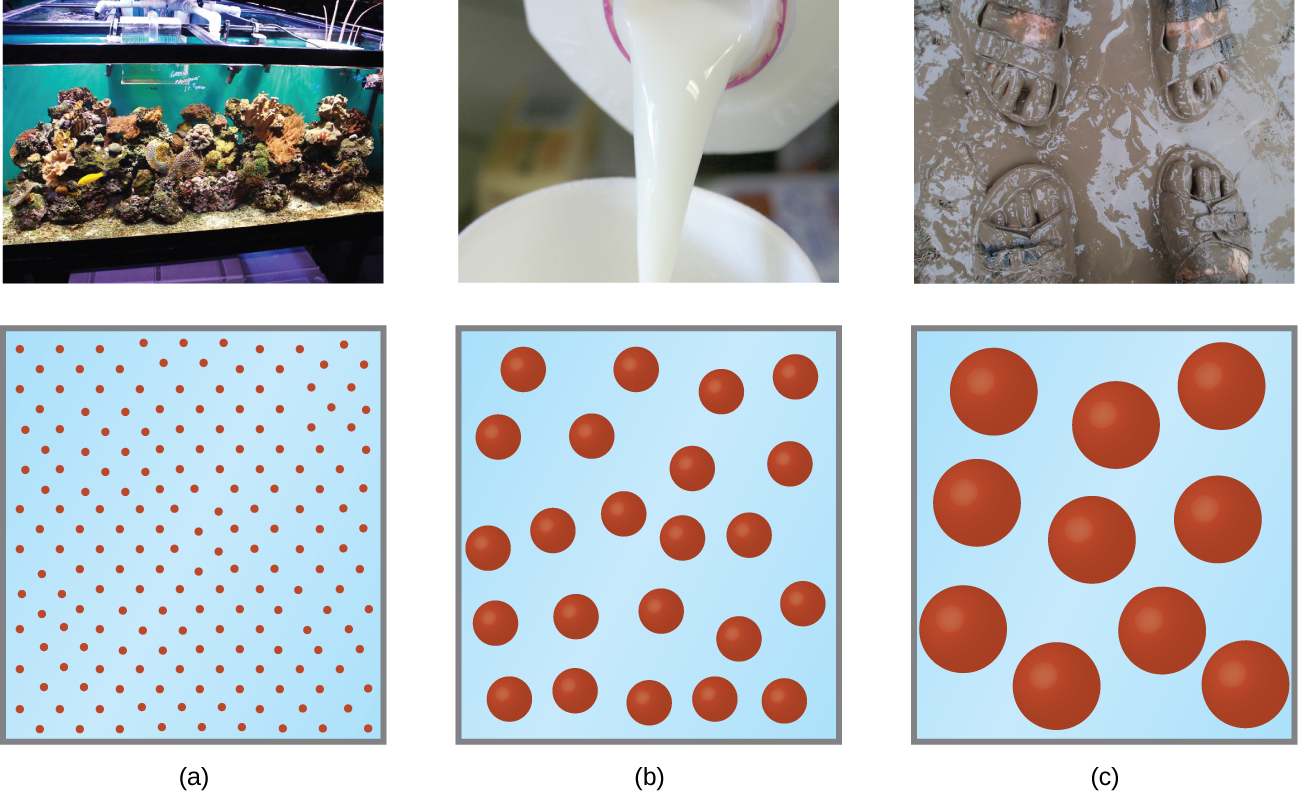
\includegraphics[scale=0.8]{Colloid.png}
\caption[Dissolucions, suspensions i col·loides]{(a) Una dissolució és una mescla homogènia, com l'aigua salada de l'aquari. (b) En un col·loide les partícules són més grans, però es mantenen disperses i no precipiten (llet). (c) Una suspensió és una mescla heterogènia amb particules que poden acabar precipitant. (adaptat de \citep{fernandez-nieves_fluids_2016})}
\label{fig:Colloid}
\end{figure}

\begin{table}[h!]
  \begin{center}
    \caption{Diferents tipus de dispersions}
    \label{tab:colloid}
    \begin{tabular}{l|l|l|l}
      & \multicolumn{3}{c}{Dispersant}\\ 
      \hline
      Dispers & Sòlid & Líquid & Gas\\
      \hline
      Sòlid & Alguns al·liatges; gemmes acolorides & Gels o suspensions (pintures) & Aerosols (fum) \\
      Líquid & Geles (gelatina) & Emulsions & Aerosols (boira) \\
      Gas & Escuma aïllant & Escuma (cervesa) & \\
      \hline
    \end{tabular}
  \end{center}
\end{table}
\item La \emph{matèria homogènia} és aquella que és idèntica quant a composició i propietats sigui quina sigui la porció que n'agafem. L'aigua de mar, la sal o un lingot d'or en són exemples:
\begin{itemize}
\item L'aigua de mar és una \emph{dissolució}, en tant que formada per dos o més components. Les propietats d'una dissolució poden ser radicalment diferents de les dels seus components: aigua i sal no són conductors de l'electricitat, però la seva dissolució ho és. Les dissolucions són homogènies a la subdivisió, però heterogènies al canvi d'estat. Els components no es poden barrejar en qualsevol proporció (per exemple, la solubilitat depèn de la temperatura). Les propietats depenen de la concentració, com mostra la Figura \ref{fig:watsuc2} (temperatura d'ebullició o fusió de l'aigua amb sals o anticongelants).
\begin{figure}[h]
\centering
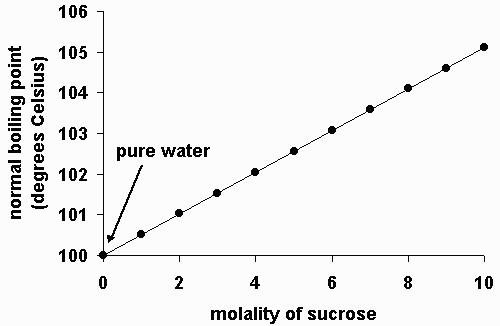
\includegraphics[scale=0.8]{watsuc2.png}
\caption{La temperatura d'ebullició d'una dissolució aquosa es modifica en funció de la concentració de solut.}
\label{fig:watsuc2}
\end{figure}
\item La sal i l'or són \emph{substàncies pures}, en tant que formades per un sol component i amb propietats físiques i químiques característiques d'aquests (densitat, temperatura de fusió o d'ebullició, solbilitat en un dissolvent donat, índex de refracció, viscositat, etc).
\end{itemize}
\end{itemize}


La Figura \ref{fig:SeparacioMescles} mostra un resum esquemàtic dels processos per reduir la complexitat d'una determinada mescla.

\begin{figure}[h]
\centering
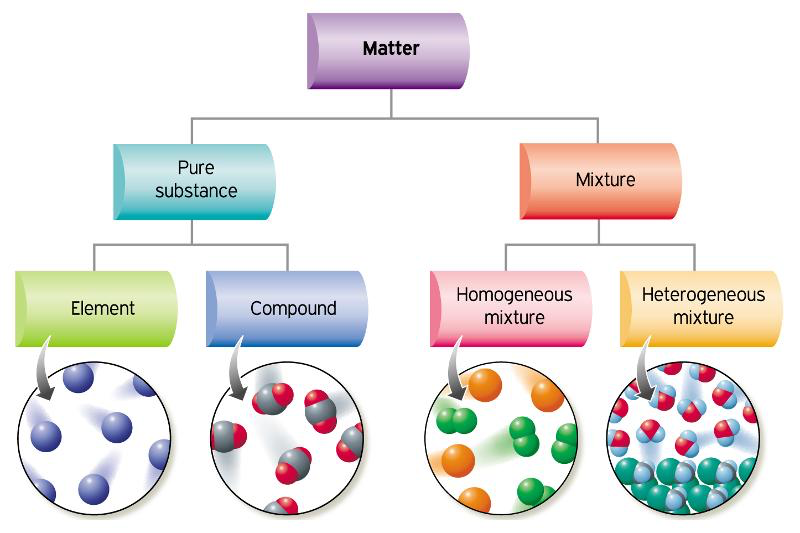
\includegraphics[scale=0.35]{Mixtures.png}
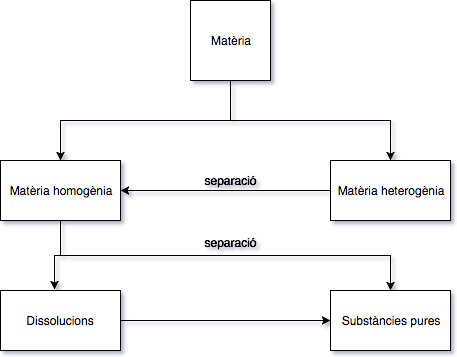
\includegraphics[scale=0.50]{SeparacioMescles.png}
\caption{Classificació de la matèria (adaptat de \citep{caamano_ros_quimica_1991})}
\label{fig:SeparacioMescles}
\end{figure}

Algunes tècniques de separació:
\begin{itemize}
\item mètodes simples de separació de mescles: filtració, decantació, centrifugació, cristal·lització, destilació, etc;
\item mètodes per separar mescles de múltiples components: 
\begin{itemize}
\item cristal·lització fraccionada (dos sòlids amb solubilitats diferents);
\item destil·lació fraccionada (dos líquids de punts d'ebullició semblants amb columnes de fraccionament, veure Figura \ref{fig:Crude_Oil_Distillation_Unit});
\item cromatografia (d'adsorció, de repartiment, d'intercanvi iònic, de filtració sobre gels); sobre paper, de columna, sobre capa fina...; gas-sòlid, líquid-líquid, gas-líquid.
\end{itemize}  
\begin{figure}[h]
\centering
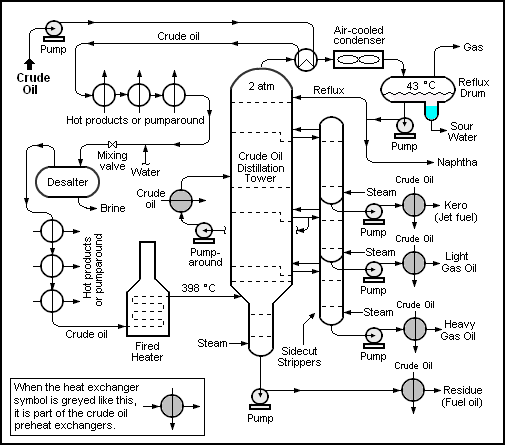
\includegraphics[scale=0.8]{Crude_Oil_Distillation_Unit.png}
\caption{Esquema de la columna de destilació del petroli.}
\label{fig:Crude_Oil_Distillation_Unit}
\end{figure}
\end{itemize}

Per a caracteritzar la puresa d'una substància, analitzem les seves propietats característiques mitjançant tècniques molt diverses, entre elles l'anàlisi dels seus espectres:
\begin{itemize}
\item espectroscopia infraroja (IR), 
\item espectroscopia visible i ultraviolada (UV)
\item espectroscopia de resonància magnpetica nuclear (NMR)
\item difracció de raigs X
\item espectroscopia de masses
\item etc
\end{itemize}

\subsection{Elements i compostos}

Els \emph{compostos} es poden descomposar en substàncies més simples. En canvi, els \emph{elements} o substàncies simples són indivisibles. Addicionalment, un compost es pot sintetitzar a partir de substàncies més simples, cosa que no passa amb els elements (Figura \ref{fig:CompostosElements}). 

Robert Boyle va donar la primera definició d'Element l'any 1661. Lavoisier va donar una llista d'elements coneguts el 1789 però hi va incloure la llum i la calor. També va formular la llei de la conservació de la massa. El 19800, Alessandro Volta va inventar la pila elèctrica i va permetre separar nous elements (electròlits) per part de Humphry Davy el 1807: el sodi i el potassi. El mateix 1807, Dalton publica la seva teoria atòmica.

Es poden combinar els elements de qualsevol manera per formar compostos? Ho veurem a la secció següent.

\begin{figure}[h]
\centering
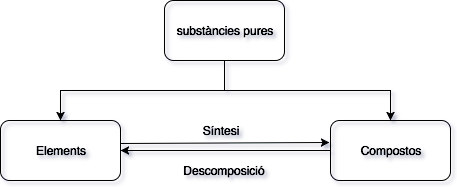
\includegraphics[scale=0.8]{CompostosElements.png}
\caption{Relació entre compostos i elements.}
\label{fig:CompostosElements}
\end{figure}


\section{La naturalesa atòmica de la matèria}

Durant molts anys l'observació de fenòmens químics senzills va servir per determinar les lleis fonamentals de la química que la van distingir de l'alquímia.

\begin{mdframed}[backgroundcolor=gray!30,frametitle=Llei de les proporcions definides]
En un compost donat, els elements constituients es combinen sempre en les mateixes proporcions pondarebles, sigui quin sigui l'origen i el mode de preparació dels compostos.
\end{mdframed}

Veurem que a cada element se li pot assignar un pes determinat i això fa que la seva combinació dongui un pes determinat i una fórmula determinada als compostos.
Per exemple, si pensem en l'òxid nítric, \ch{NO} i mirem d'augmentar el mínim possible (un àtom d'oxigen o un de nitrogen) arribem a nous compostos molt diferents de l'inicial i entre ells, \ch{N2O} i \ch{NO2}. 

De fet, la llei és força simple i poc precisa, ja que els elements poden tenir diferents isòtops.
Els isòtops d'un element tenen diferents masses atòmiques (sempre tindran el mateix número de protons, però poden diferir en el número de neutrons). La massa atòmica promig es mesura ponderant les masses atòmiques de cada isòtop amb la seva abundància a la terra (veure Figura \ref{fig:PropietatsHidrogen}).
Els objectes extraterrestres poden tenir composicions isotòpiques molt diferents.
\begin{figure}[h]
\centering
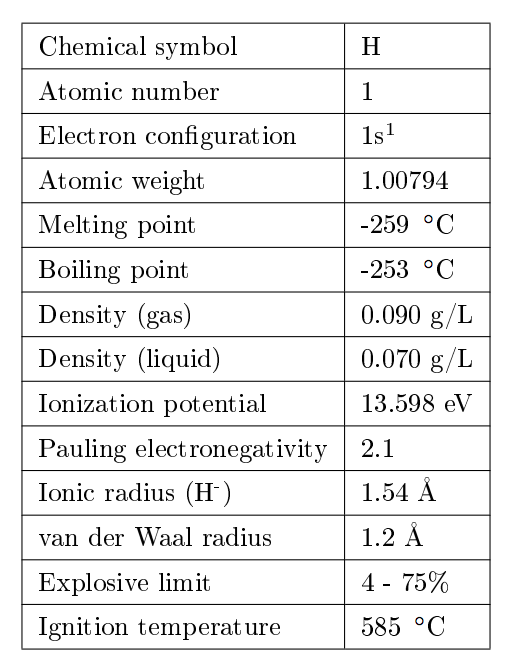
\includegraphics[scale=0.35]{PropietatsHidrogen.png}
\caption{Propietats físiques de l'àtom d'hidrogen (Adaptat de Connexions \linkurl{http://cnx.org/content/col10984/1.4})}
\label{fig:PropietatsHidrogen}
\end{figure}
\begin{exr}
Entra a \linkurl{https://teachchemistry.org/periodical/issues/may-2017/isotopes-calculating-average-atomic-mass} i calcula la massa atòmica promig d'alguns elements.
\end{exr}
També es viola aquesta llei en alguns sòlids iònics com l'òxid de zinc, el sulfur cuprós (entre \ch{Cu_{1.7}S} i \ch{Cu2S}) o l'òxid ferrós.

Els compostos sòlids que no estan formats per molècules definides presenten característiques diferents. Podem preparar cristalls de \ch{TiO}, però variant les condicions de preparació podem anar de \ch{Ti_{0.75}O} a \ch{TiO_{0.69}}, encara que la seva estructura espaial sigui idèntica. Es tracta de compostos no estequiomètrics i, tot i que no varïin les seves propietats estrcuturals, sí que ho fan les òptiques o la resistivitat (veure Figura \ref{fig:TiOPhaseDiagram}).
\begin{figure}[h]
\centering
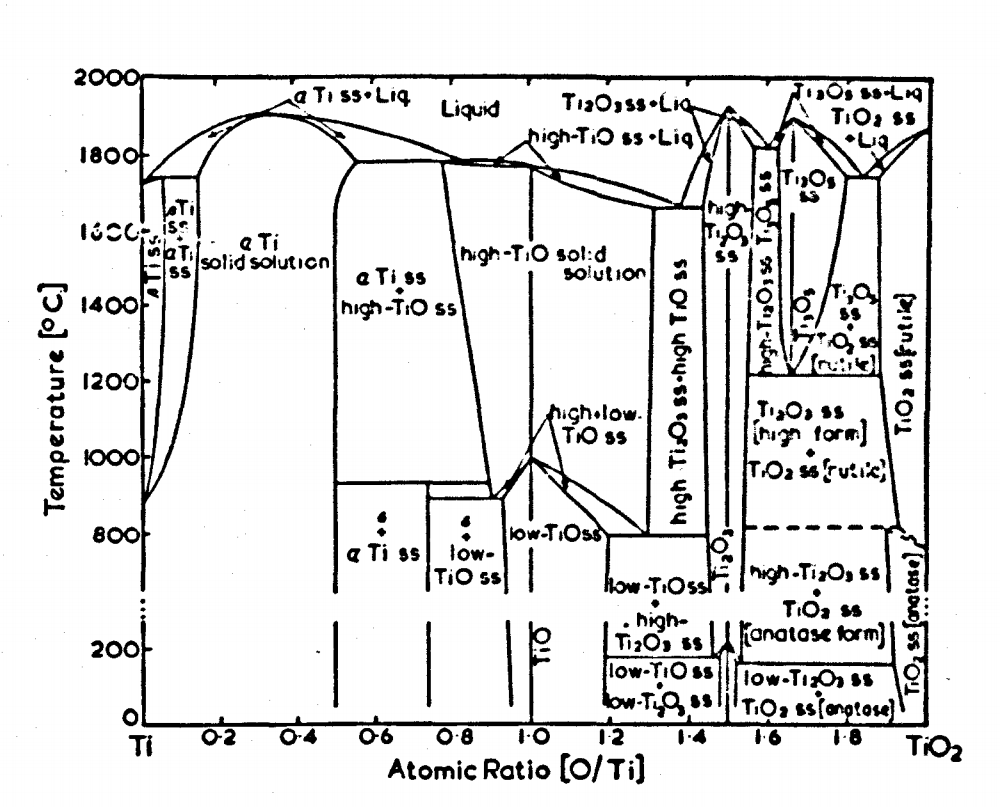
\includegraphics[scale=0.35]{TiOPhaseDiagram.png}
\caption{Diagrama de fase de l'òxid de titani en diverses composicions (no)estequiomètriques\citep{de_vries_phase_1954}}
\label{fig:TiOPhaseDiagram}
\end{figure}

\begin{mdframed}[backgroundcolor=gray!30,frametitle=Llei de les proporcions múltiples]
Si dos elements formen més d'un compost, els diferents pesos d'un d'ells que es combinen amb el mateix pes de l'altre, estan en una relació de números enters petits.
\end{mdframed}

Els diferents òxids del nitrogen en són un bon exemple: amb 16g d'oxigen es poden combinar 28, 14 o 7 grams de nitrogen (proporció 4:2:1)

\begin{mdframed}[backgroundcolor=gray!30,frametitle=Llei de les proporcions equivalents]
Si una determinada quantitat de l'element C reacciona amb una quantitat donada de l'element A, p$_A$, i una donada de l'element B, p$_B$, A i B reaccionen en una proporció que és múltiple simple o fracció de números sencers de la raó p$_A$/p$_B$.
\end{mdframed}

El nitrogen i l'oxigen reaccionen amb l'hidrogen per formar amoniac (\ch{NH3}) i aigua (\ch{H2O}), respectivament. 1g d'hidrogen reacciona amb 4,66g de Nitrògen per formar amoniac i amb 8 grams d'oxigen per formar aigua. Per tant, 4.66/8.00=0.583.
En el cas de la reacció \ch{N2 + O2 -> 2NO}, 28g de nitrogen reaccionen amb 32g d'oxigen. 28/32=0.875, que és 1.5 vegades 0.583 o, el que és el mateix, la fracció 3/2.



\subsection{Pesos atòmics i fòrmules moleculars (M)}

En principi, doncs, era possible relacionar els pesos de tots els elements i la manera en què es combinaven. El problema és que no es tenia cap certesa sobre cap compost inicial, ni sobre cap pes atòmic. Dalton no podia fer més que conjectures.

Gay-Lussac va mostrar el volum de la combinació de dues substàncies estava relacionat amb números sencers, com també marcava la llei de proporcions múltiples. Entre aquesta observació i l'admissió de que els elements nitrogen i oxigen podien ser poliatòmics, va dur Amedeo Avogadro (1811) es van acostar a la determinació dels pesos moleculars, però encara hi havia indeterminació. Finalment, Cannizaro va crear l'escala de pesos a partir de l'observació que la teoria atòmica de Dalton establia que el níumero d'àtoms en una molècula havia de seguir proporcions senceres. Va establir el pes de l'hidrogen com a 2g.

Per ser més precisos en la determinació de pesos atòmics es poden usar altres tècniques. Per exemple, considerant que a temperatura 0K els gasos es comporten de manera ideal i la densitat és proporcional a la pressió ($\delta=\alpha P$, on $\alpha$ seria la densitat que tindria un gas ideal a pressió 1 atm) però que a pressions més elevades cal millorar aquesta aproximació ($\delta = \alpha P + \beta P^2$), podem graficar $\delta/P$ en funció de la $P$ i obtindrem línies rectes com la de la Figura \ref{fig:DensitatIdealCO2}.
\begin{figure}[h]
\centering
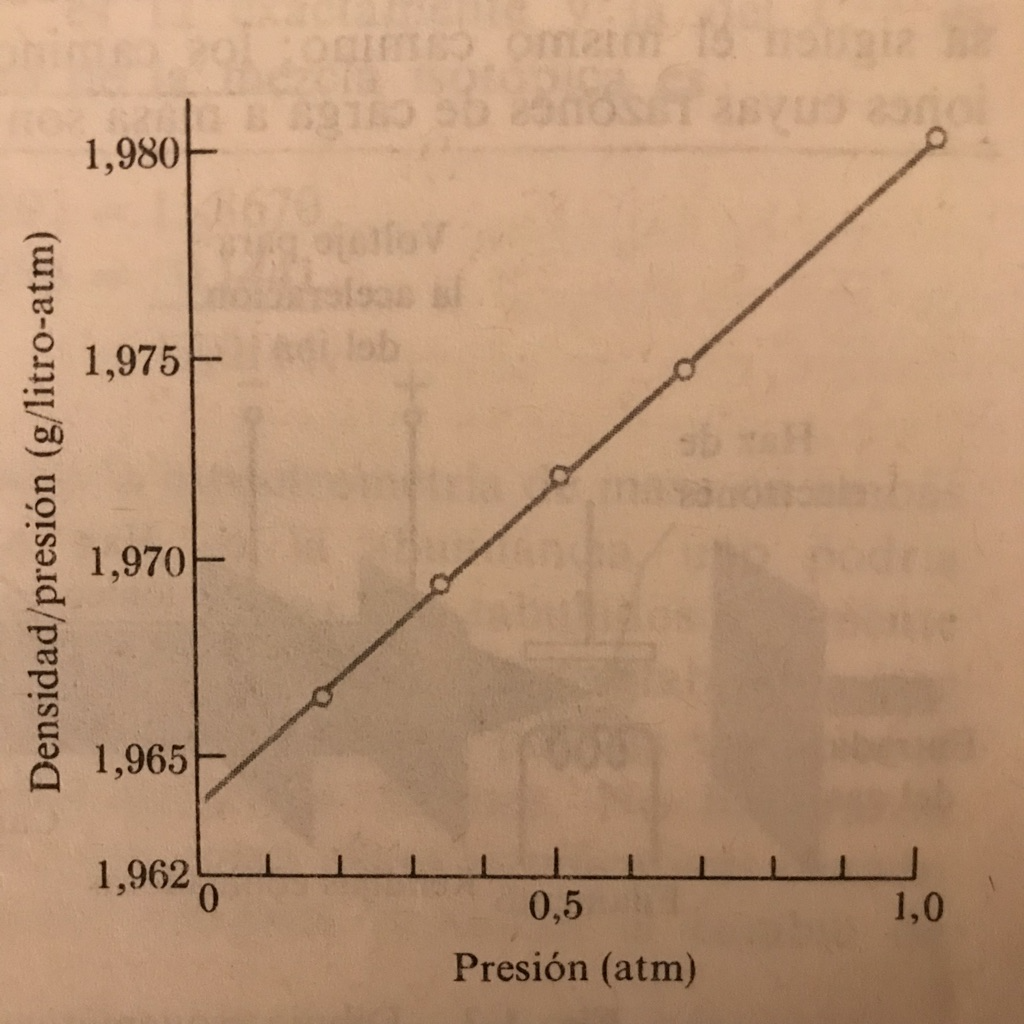
\includegraphics[scale=0.3]{DensitatIdealCO2.png}
\caption{Determinació de la densitat ideal del \ch{CO2} a 273,1$^{\circ}$K.}
\label{fig:DensitatIdealCO2}
\end{figure}
\begin{exr}
Si la densitat del gas oxigen és de 1.428g/l a 1atm i 273.1K i la del \ch{CO2} és 1.9635g/l a les mateixes condicions, i si el pes molecular de l'oxigen és 31,998, quin és el pes molecular del \ch{CO2}?
\end{exr}

\begin{mdframed}[backgroundcolor=gray!30,frametitle=Concepte de mol]
El número d'àtoms de carboni contingut en, exactament, 12g de \ch{C^{12}} s'anomena número d'Avogadro, \emph{N}. Un mol és la quantitat de matèria que conté el número d'Avogadro de partícules.
\end{mdframed}

\newpage

\subsection{Estequiometria (M)}

\section{Gasos}
\label{sec:gasos}

Dels gasos podem mesurar una sèrie de propietats característiques que ens permeten el seu estudi precís: \textbf{massa}, \textbf{volum}, densitat, \textbf{pressió}, \textbf{temperatura}, compressibilitat, coeficient de dilatació tèrmica, capacitat calorífica, viscositat, conductivitat tèrmica, difusivitat, etc, de les quals hem remarcat les anomenades \textbf{propietats primàries}.

La pressió es mesura en el S.I. en Pascals:
\[
1 {\rm Pa}=\frac{1 {\rm N}}{1 {\rm m}^2}
\]
però es treballa sovint en atmosferes (1 atm = 1.01325 $\times$ 10$^5$ Pa = 760 Torr = 760 mmHg).
\begin{figure}[h]
\centering
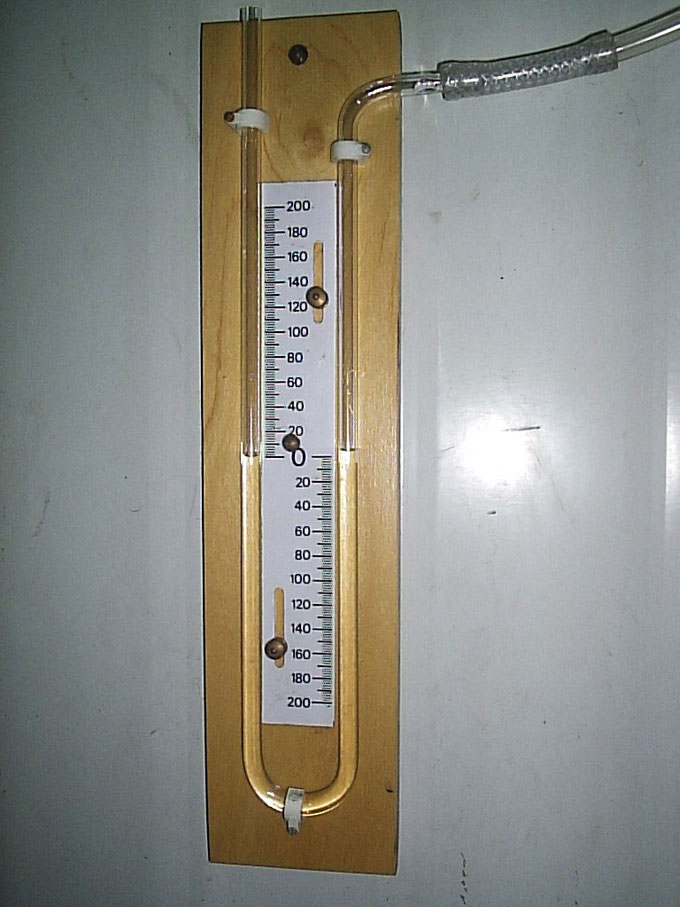
\includegraphics[scale=0.33]{Manometre.png}
\caption[Manòmetre diferencial]{Un manòmetre diferencial mesura la diferència entre les pressions externes i d'un determinat gas. Cal tenir en compte la pressió atmosfèrica exterior (approx 1 atm).}
\label{fig:Manometre}
\end{figure}
Les equacions que depenen de les quatre propietats primàries s'anomenen equacions d'estat:
\[F(p,m,V,T)=0\]
En situacions normals (absència de camps elèctrics externs, per exemple) tres de les propietats són suficients per determinar la quarta (10g de N$_2$ a 30$\degree$C no podem saber en quin estat es troben -spolid, líquid o gas- ja que ens manca conèixer la pressió, i així en qualsevol situació).

D'altra banda, les propietats es poden classificar entre extensives (m, V, ...) o intensives (T, P, capacitat calorífica ...), segons depenguin de la quantitat de substància o no. La raó entre dues propietats extensives és sempre intensiva: $\delta = \frac{m}{V}$; $\nu = \frac{V}{m}$. Només necessitem dues propietats intensives per determinar l'estat d'un gas ($P$ i $T$) i, per tant, amb tres variables intensives podem construir una equació d'estat: 
\[F(p,V_{\rm m},T)=0\]

La mesura d'una propietat per mol sanomena valor molar d'aquesta variable: $V_{\rm m} = \frac{V}{n}$. 
\subsection{Llei de Boyle}

Robert Boyle (1627-1691) va notar, fent servir un manometre com el de la Figura \ref{fig:Manometre}, que existia una determinada llei de proporcionalitat entre la pressió exercida sobre un gas i el volum d'aquest
\begin{figure}[h]
\centering
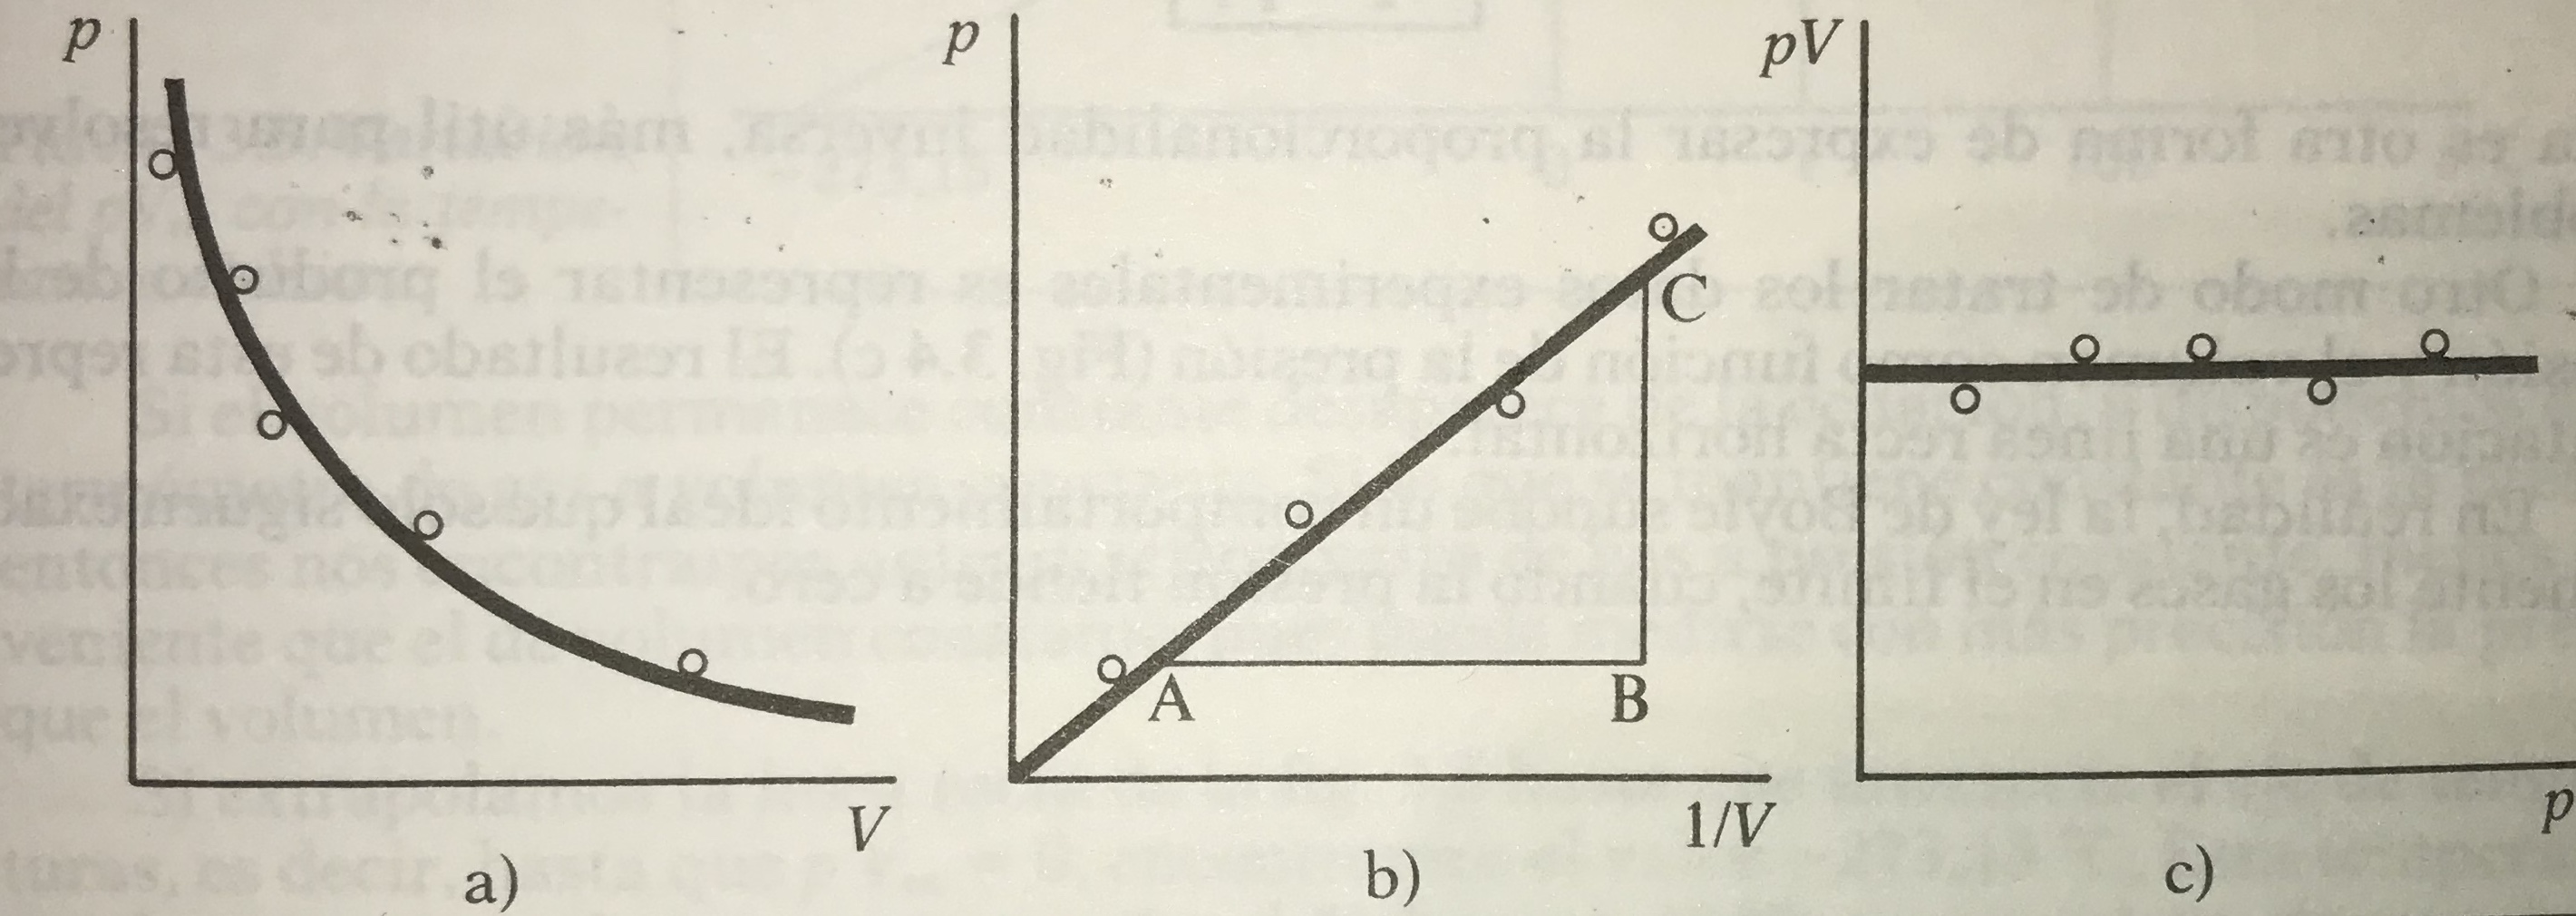
\includegraphics[scale=0.10]{Boyle.png}
\caption{Experiment de Boyle i llei de proporcionalitat entre la pressió exercida sobre un gas i el seu volum.}
\label{fig:Boyle}
\end{figure}
Va descobrir que el producte entre el volum i la pressió és una constant, la qual cosa duu a que sota dues condicions diferents de pressió els volums es comporten de la següent manera per al mateix gas a una temperatura donada:
\[
\frac{V_1}{V_2}=\frac{P_2}{P_1}
\]


\subsection{Llei de Charles i Gay-Lussac}

JAcques Charles (1787) i posteriorment Gay-Lussac van trobar que per a una mateixa pressió, la relació $\frac{V_{100 \degree C}}{V_{0 \degree C}}$ era identica per a tots els gasos (1.376).

Això duu a extrapolar fàcilment el comportament dels gasos i determinar el zero absolut de temperatura segons el gràfic \ref{fig:zeroabsolut}. Lord Kelvin (1848) va proposar usar el punt d'intersecció del gràfic amb la línia de les abcisses com a origen d'una nova escala de temperatura: $T/\rm{K} = t/\degree \rm{C} + 273.15$.\marginnote{en realitat s'usa 273.16, que és el punt triple de l'aigua, temperatura a la qual coexisteixen en equilibri aigua, gel i vapor en un recipient tancat}
\begin{figure}[h]
\centering
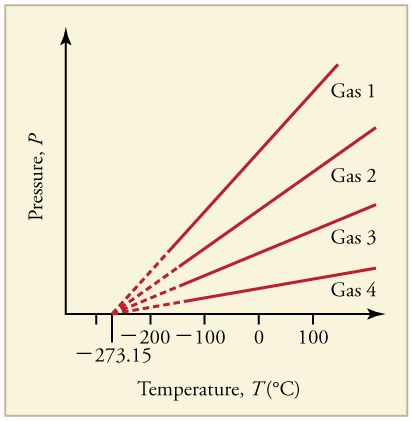
\includegraphics[scale=1.0]{zeroabsolut.png}
\caption{Gràfic del zero absolut a partir de la llei de Charles i Gay-Lussac.}
\label{fig:zeroabsolut}
\end{figure}

De la nova llei es desprèn que 
\[\frac{P V_{\rm m}}{T}= cnt = R\]
o bé
\[P V = n R T\]
que es coneix com a equació d'estat d'un gas ideal.

\subsection{Gas ideal}

Per tal de determinar la $R$ no podem simplement calcular el quocient $\frac{P V_{\rm m}}{T}$ per a qualsevol gas, ja que cadascun d'ells donarà un valor diferent (només és vàlida l'expressió per a un gas ideal!). Veure la Figura \ref{fig:R2}.
\begin{marginfigure}
\centering
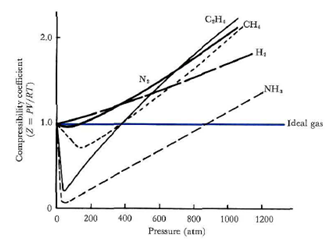
\includegraphics[scale=1.0]{R2.png}
\caption[Determinació de la constant dels gasos $R$]{R es pren com al valor límit de la fracció $\frac{P V_m}{T}$ per a tots els gasos: 
$R=\lim_{P \to 0} \frac{P V_{\rm m}}{T}= 0.08205 \frac{{\rm atm l}}{{\rm mol K}}$
}
\label{fig:R2}
\end{marginfigure}

\begin{exr}
Calcular el volum molar d'un gas ideal a condicions normals (1 atm i 0$\degree$C).
\end{exr}

\begin{exr}
Quant gas hi ha en una mostra de volum 0.5 dm$^3$, a 80 graus Celsius i 800 Torr de pressió?.
\end{exr}

\begin{exr}
Un conductor comprova la pressió dels pneumàtics pel matí aviat, quan la temperatura és de 15$\degree$C, i és de 1.3$\times$10$^5$ Pa. Al migdia la temperatura és 15 graus més elevada. Quina és la pressió dels pneumàtics ara?.
\end{exr}

\begin{exr}
Si a CN la densitat d'un gas ideal és de 1.62 g dm$^{-1}$, quina és la seva massa molar? i quina densitat tindrà a 300 K i 2.4$\times$10$^5$ Pa?.
\end{exr}

\begin{exr}
Dalt de l'Everest, la pressió atmosfèrica és de 0,33 atm i la temperatura de 50 sota zero. Quina és la densitat de l'aire i en CN és de 1.29 g dm$^-3$?.
\end{exr}

\subsection{Teoria cinètica dels gasos (M)}

Per tal de relacionar aquestes descobertes amb l'estructura atòmica de la matèria, ens cal pensar una teoria que representi els gasos de forma extremadament simple: un \textit{model}. En el nostre cas (veure Figura \ref{fig:TeoriaCinetica}),
\begin{itemize}
\item el gas es format per partícules que es comporten com a punts de massa,
\item que llevat no col·lideixin no exerceixen força els uns sobre els altres
\end{itemize}
\begin{figure}[h]
\centering
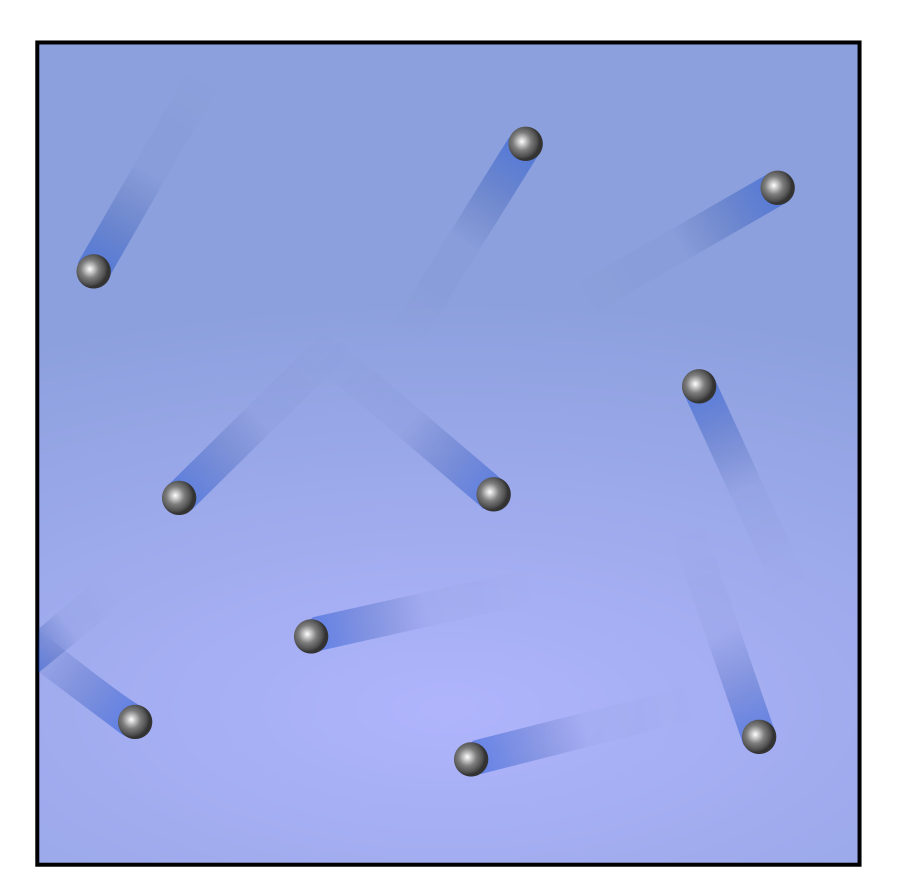
\includegraphics[scale=0.2]{TeoriaCinetica.png}
\caption{Representació del moviment de les partícules en un gas ideal.}
\label{fig:TeoriaCinetica}
\end{figure}
\begin{exr}
Pots calcular el volum ocupat per molècula en un gas ideal a CN?. Es troben dues molècules molt freqüentment en un gas a baixa pressió?
\end{exr}
Aquesta teoria, de forma relativament simple, ens permet expressar la pressió que s'exercexi sobre les parets d'un recipient per part del gas que conté segons:
\[
PV=\frac{2}{3} \left< E_c \right> = \frac{2}{3} \left< \frac{mc^2}{2} \right>
\]

D'aquí s'extreuen resultats interessants, com que l'energia cinètica translacional d'un mol de gas és \[N_0 \frac{m <c^2>}{2}=\frac{3}{2} RT\] o bé, si dividim pel número d'Avogadro a esquerra i dreta obtenim la constant dels gasos per molècula a partir de l'energia cinètica per molècula (constant de Boltzmann $k$): \[\frac{m <c^2>}{2}=\frac{3}{2} kT\].
Aquest resultat ens diu que si dos gasos tenen la mateixa $T$, les seves molècules tenen la mateixa energia cinètica promig. 
\begin{exr}
Qui es mou més ràpid, una molècula d'oxigen o una de nitrogen en dues mostres d'aquests gasos a la mateixa temperatura? Pots explicar perquè la pressió és independent de la natura de les molècules?
\end{exr}

\begin{exr}
Calcula la velocitat mitjana de les molècules d'hidrògen a 25$\degree$C.
\end{exr}

La distribució de les velocitats de les partícules d'un gas segueix la distribució de Maxwell-Boltzmann:
\[
\frac{\Delta N}{N}=4 \pi \left( \frac{m}{2 \pi kT}\right)^{3/2} \underbrace{e^{-mc^2/2kT}}_{\rm Boltzmann} c^2 \Delta c
\]
El factor de Boltzmann ens diu, en aquesta equació, que a qualsevol temperatura particular, acostuma a haver moltes menys molècules amb energies altes que amb energies baixes.
\begin{figure}[h]
\centering
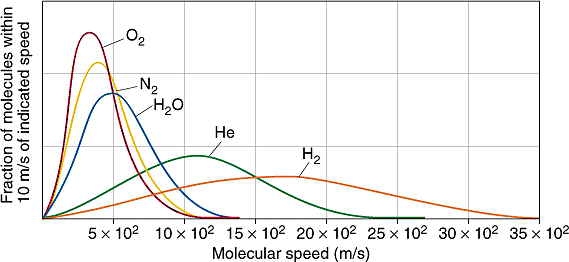
\includegraphics[scale=0.5]{BolzDist.png}
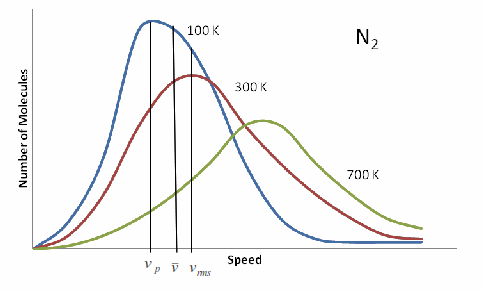
\includegraphics[scale=0.5]{MXDIST.png}
\caption{La distribució de Maxwell per a diferents molècules i temperatures}
\label{fig:TeoriaCinetica}
\end{figure}

\subsection{Capacitat calorífica}

La capacitat calorífica d'una substància és la quantitat de calor en calories necessària per elevar 1$\degree$C la temperatura d'un gram de la substància.

De fet, això necessita precissió: no és el mateix fer aquest procés dpescalfament a volum constant que a pressió constant ($C_V$ vs $C_P$).

Si afegim calor a un gas, o bé s'expandeix (i per tant fa treball) o bé la velocitat de les seves particules augmenta.
A $V$ constant, l'escalfament produeix un increment d'energia cinètica:
\[\Delta E = \frac{3}{2} R \Delta T\]
però resulta que $\Delta E/ \Delta T$ és, justament, $C_V$ i, per tant, per a un gas monoatòmic ideal, $C_V=\frac{3}{2}R$ o, aproximadament, 3 cal/mol·grau.

En el cas de pressió constant, les partícules augmenten la seva energia cinètica i també exerceixen treball ($\Delta(PV)$):
\[\Delta(PV)=P\Delta V = P(V_2-V_1)=PV_2-PV_1\]
Per a un mol de gas, resulta que $PV=RT$ i, per tant, 
\[PV_2-PV_1=RT_2-RT_1=R\Delta T\]
Per tant, la capacitat calorífica extra pel fet de fer el procés a pressió constant és
\[\frac{\Delta (PV)}{\Delta T}=R\]
i, per tant, 
\[C_P=C_V+R 
=\frac{3}{2} R + R= \frac{5}{2}R\]
És fàcil veure que $C_P/C_V=5/3=1.67$ i podem comparar aquests coeficients per a diversos gasos reals, per tal d'establir diferències amb el seu comportament ideal (\ref{tab:cpcv}).
\begin{margintable}
  \begin{center}
    \caption{Quocients de capacitat calorífica \citep{mahan_quimica_1997}}
    \label{tab:cpcv}
    \begin{tabular}{cc|cc}
      \hline
      Gas & $C_P/C_V$ & Gas & $C_P/C_V$\\
      \hline
      He & 1.66 & \ch{H2} & 1.41 \\
      Ne & 1.66 & \ch{O2} & 1.40 \\
      Ar & 1.66 & \ch{N2} & 1.40 \\
      Kr & 1.66 & \ch{CO} & 1.40 \\
      Xe & 1.66 & \ch{NO} & 1.40 \\
      Hg & 1.66 & \ch{Cl2} & 1.36 \\
      \hline
    \end{tabular}
  \end{center}
\end{margintable}
\begin{exr}
Perquè hi ha aquestes diferències entre la columna de l'esquerra i la de la dreta de la Taula \ref{tab:cpcv}? (Adona't que si un gas monoatpomic ideal, pel fet d'estar només augmentant la seva energia cinètica té una $C_V=\frac{3}{2}R$, es pot entendre que per a cada component necessita $\frac{3}{2}R$)
\end{exr}




\subsection{Gasos no ideals}

En gasos reals, el factor 
\[z=\frac{V_m}{V_{m,i}}=\frac{V_m}{RT/P}=\frac{PV_m}{RT}\]
no és 1, com succeiria a un gas ideal (veure Figura \ref{fig:FactorCompress}).
\begin{figure}[h]
\centering
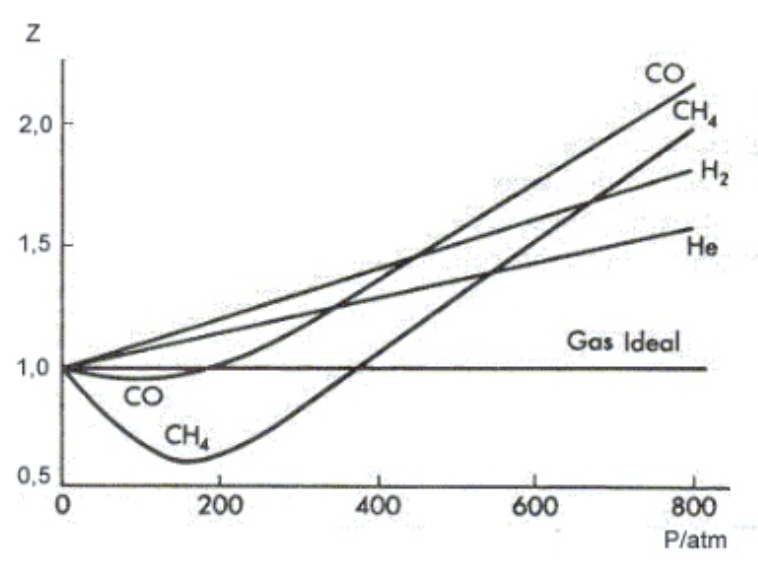
\includegraphics[scale=0.5]{FactorCompress.png}
\caption{Factor de compressibilitat per a diferents gasos a 0$\degree$C}
\label{fig:FactorCompress}
\end{figure}

Per tal de millorar l'aproximació a la realitat podem considerar diferents aproximacions. La més simple consisteix a pensar que el volum ideal explorat per les molècules és més gran que el volum que poden explorar en realitat, per un valor $b$ que prové del volum exclós per la presència d'altres molècules.
\[V_m = V_{m,i}+b=\frac{RT}{P}+b\]

Segons això,
\[z=\frac{PV_m}{RT}=1+\frac{b}{RT}P\]
que té una forma lineal. Aixó explicaria el cas de la molècula d'hidrogen.
Però què passa amb \ch{CH4} o \ch{CO}? Val la pena pensar que són molècules que es podran trobar líquides a temperatures més baixes amb major facilitat que no pas \ch{H2}. En un gas real, la pressió que exerciran les molècules sobre la paret del recipient serà més baixa que en un gas ideal:
\[P=P_i -\Delta P\]
Es pot veure que aquest increment de pressió és proporcional al quadrat de la concentració ($c=\frac{m}{V}=\frac{1}{V_m}$):
\[\Delta P \alpha c^2 \alpha \frac{1}{{V_m}^2} \]
o bé
\[\Delta P = \frac{a}{{V_m}^2}\]
i, per tant, 
\[ P_i=P+\frac{a}{{V_m}^2}\]

Si ara substituïm el volum i pressió ideals en l'equació dels gasos ideals:
\[
\left( P + \frac{a}{{V_m}^2} \right) (V_m -b)=RT
\]
o bé
\begin{equation}
\left( P + \frac{n^2 a}{V^2} \right) (V -nb)=nRT
\label{Eq:vdW}
\end{equation}

\begin{exr}
Què passa segons l'Equació \ref{Eq:vdW} si la pressió es fa propera a zero o bé la temperatura es fa molt gran per a un gas real? (veure la Figura \ref{fig:FactorCompressT}).
\end{exr}

\begin{figure}[h]
\centering
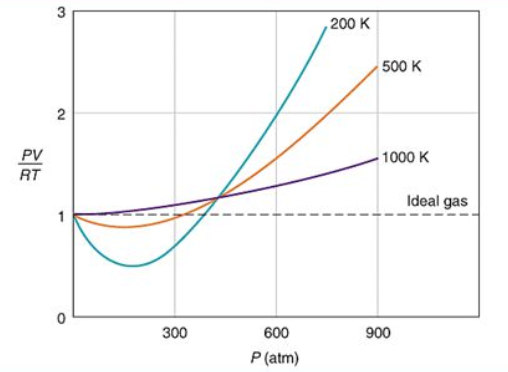
\includegraphics[scale=1.0]{FactorCompressT.png}
\caption{Factor de compressibilitat per a un mateix gas a diferents temperatures}
\label{fig:FactorCompressT}
\end{figure}

Les forces de van der Waals que fan que es perdi la idealitat són degudes a tres contribucions:
\begin{enumerate}
\item Efecte d'orientació: forces dipol-dipol.
\item Efecte de distorsió: forces d'inducció.
\item Efecte de dispersió: forces de dispersió.
\end{enumerate}

\begin{exr}
Perquè \ch{CO2} i \ch{O2} tenen una desviació negativa respecte al comportament del gas ideal a pressions i temperatures moderades, mentres que l'He i el \ch{H2} presenten una deviació positiva en les mateixes condicions?
\end{exr}


%\subsection{Fenòmens de transport (M)}



\section{Sòlids}
\subsection{Propietats (M)}

Es caracteritzen per la seva rigidesa, incompressibilitat i per les seves característiques geomètriques.
La teoria atòmica ens ajuda a entendre el seu comportament basat en l'estructura d'una xarxa cristalogràfica.



\subsection{Tipus (M)}

Podem distingir:
\begin{description}
\item[sòlids cristal·lins] Exemples: clorur sòdic, sofre... 
\begin{itemize}
\item Són anisotròpics (la refracció, la conductivitat elèctrica, etc, depenen de la direcció en la qual es mesurin). 
\item Tenen punts de fusió ben definits. 
\item Es presenten a la natura sota formes polièdriques limitades per cares planes.
\end{itemize}
\item[substàncies amorfes] Exemples: vidre, plàstic... \begin{itemize}
\item No tenen caracterìstiques regulars. 
\item Són isotròpics. 
\item No estan ben establerts (són progressius) els seus punts de fusió.
\end{itemize}
\end{description}
Tots dos tipus de substàncies tenen alguna mena d'interacció local d'enllaç, però en el cas dels sòlids amorfs no existeix cap cel·la unitat.

La formació dels cristalls és depenent de la temperatura i la velocitat del procés en què es formen. Processos lents impliquen cristalls més grans, per exemple.

Els cristalls es poden estudiar per difracció de raigs X, que es basa en el fet que la longitud d'ona dels raigs X és similar a l'espaiat dels àtoms en el cristall. 

\begin{table}[h!]
  \begin{center}
    \caption[Sistemes cristal·lins i retícules de Bravais]{Sistemes cristal·lins i retícules de Bravais (veure Figura \ref{fig:Bravais}). P: centrada en les cantonades; I: centrada en el cos; F: centrada en la cara; C: amb punt central (adaptat de \citep{yen_chemistry_2008}).}
    \label{tab:Bravais}
    \begin{tabular}{cccc}
      \hline
      Sistema & Cel·la unitat & retícula de Bravais \\ 
      \hline
	  Cúbic      & $a=b=c$ & P,I (Fig. \ref{fig:crystal_structure}b),F (Fig. \ref{fig:crystal_structure}a)\\
	             & $\alpha=\beta=\gamma=90\degree$ & \\
	  Tetragonal & $a=b\neq c$ & P,I \\
	             & $\alpha=\beta=\gamma=90\degree$ & \\
	  Ortoròmbic & $a\neq b\neq c$ & P,I,C,F\\
	             & $\alpha=\beta=\gamma=90\degree$ & \\
	  Romboèdric & $a=b=c$ & R(P)\\
	             & $\alpha=\beta=\gamma \neq 90\degree$ & \\
	  Hexagonal  & $a=b\neq c$ & P (Fig. \ref{fig:crystal_structure}c) \\
	             & $a=b \neq c$ & \\
	             & $\alpha = \beta = 90 \degree$ & \\
	             & $\gamma = 120\degree$ &\\
	  Monoclínic & $a \neq b \neq c$ & P,C\\
	             & $\alpha=\gamma \neq \beta$&\\
	  Triclínic  & $a \neq b \neq c$ & P\\
	             & $\alpha \neq \beta \neq \gamma$&\\
      \hline
    \end{tabular}
  \end{center}
\end{table}

\begin{figure}[h]
\centering
\includegraphics[scale=0.1]{Bravais.png}
\caption{Retícules de Bravais i relació amb els 7 típus de cel·la unitat \citep{yen_chemistry_2008}.}
\label{fig:Bravais}
\end{figure}
\begin{figure}[h]
\centering
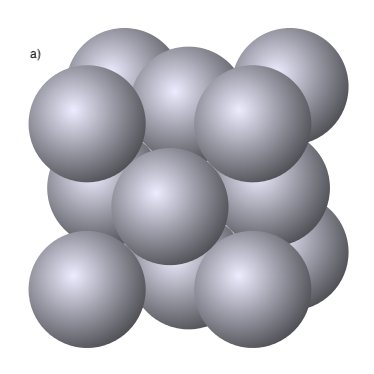
\includegraphics[scale=0.4]{FCC_crystal_structure.png}
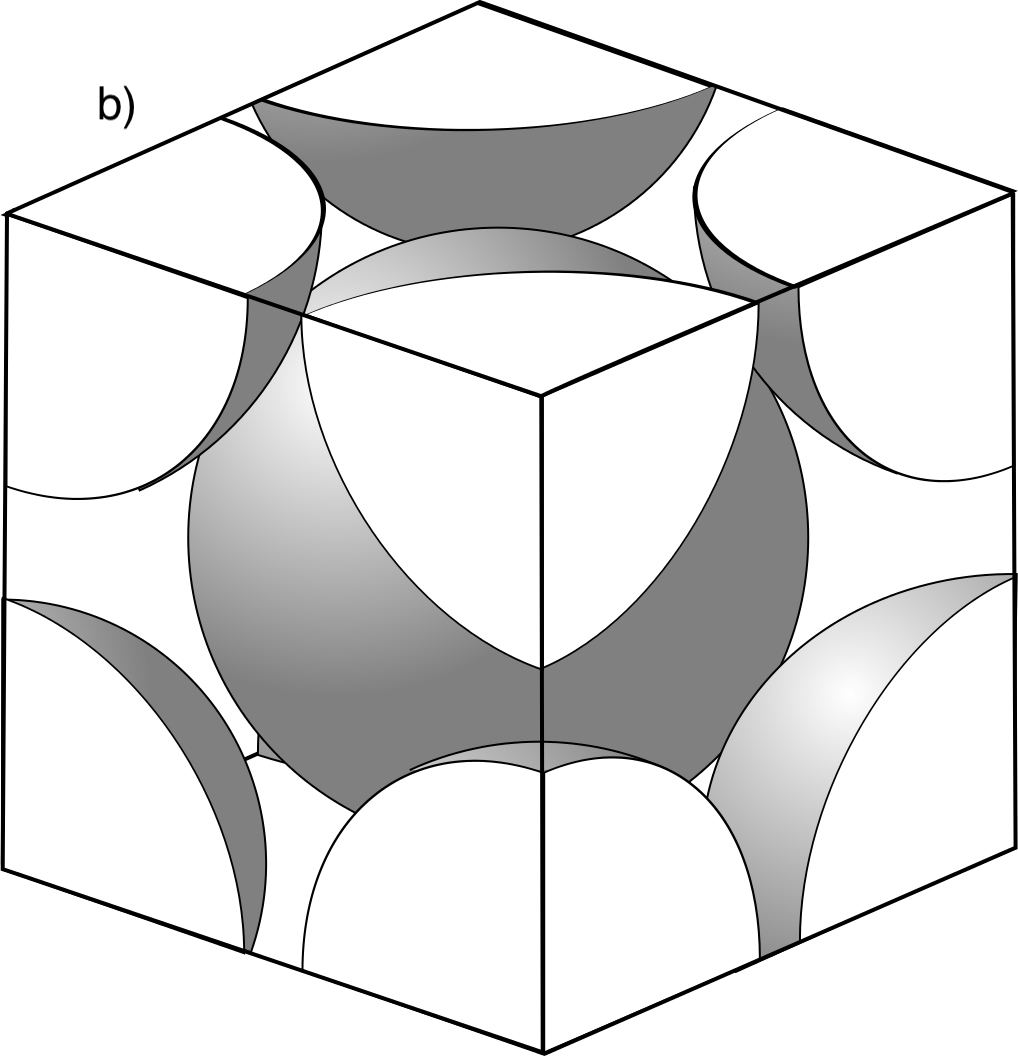
\includegraphics[scale=0.12]{CBC_crystal_structure.png}
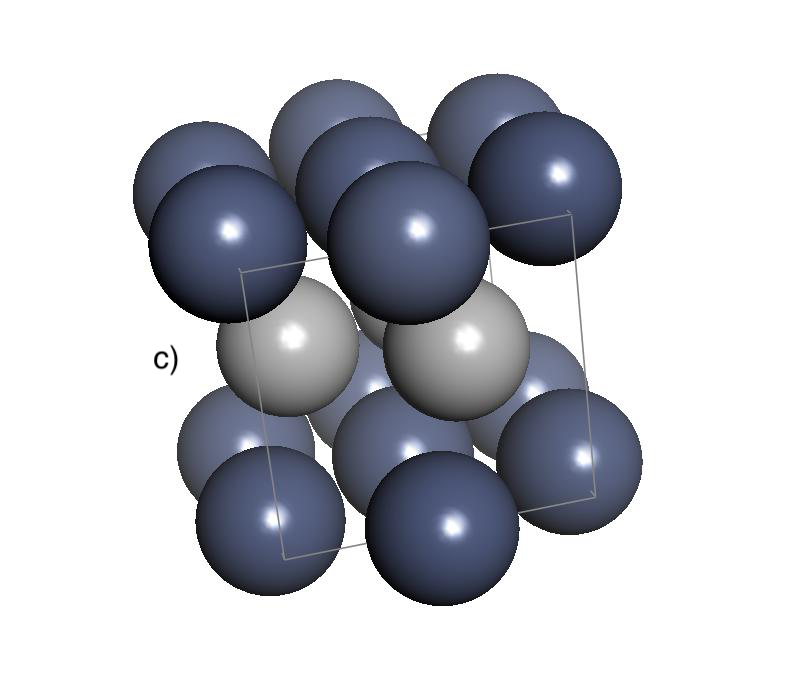
\includegraphics[scale=0.32]{HCP_crystal_structure.png}
\caption[Exemples d'estructures cristal·lines]{Exemples d'estructures: a) cel·la unitat cúbica centrada en la cara, amb 4 àtoms per cel·la unitat; b) cel·la unitat cúbica centrada en el cos; c) hexagonal (en la imatge, Hidrur de Crom, \ch{CrH_x})}
\label{fig:crystal_structure}
\end{figure}

\begin{exr}
La ratio d'empaquetament d'una cel·la unitat es defineix com la fracció entre el volum omplert pels àtoms que la formen i el seu volum total. Calcula el RE de la cel·la unitat cúbica centrada en la cara i de la cel·la unitat cúbica centrada en el cos (veure Figura \ref{fig:crystal_structure}).
\end{exr}

La Figura \ref{fig:bonding_motifs_PT} mostra els modes d'empaquetament dels elements de la taula periódica. A partir dels modes d'empaquetament també es poden calcular relacions diverses que ens indiquen el grau de direccionalitat dels enllaços entre els diferents àtoms, ajudant a identificar els diferents tipus de sòlids cristal·lins.
\begin{figure}[h]
\centering
\includegraphics[scale=0.13]{bonding_motifs_PT.png}
\caption{Estructura cristal·lina o modes d'enllaç a la taula periòdica \citep{yen_chemistry_2008}.}
\label{fig:bonding_motifs_PT}
\end{figure}

Podem distingir cinc tipus de sòlids, com es veu a la Taula \ref{tab:TipusSolids}.\marginnote{veure també \linkurl{https://chemistry.tutorvista.com/inorganic-chemistry/types-of-solids.html}}
\begin{table}[h!]
  \begin{center}
    \caption{Tipus de sòlids (adaptat de \citep{yen_chemistry_2008}.}
    \label{tab:TipusSolids}
    \begin{tabular}{llllr}
      \hline
      Tipus & Components & característiques & Exemples & Energia de cohesió \\ 
            &         &                  &          & (kJ mol$^{-1}$) \\ 
      \hline
Iònic   &  càrregues $+$ i $-$ & fràgils, aïllants             & NaCl     & 795 \\
        &                      & alt punt de fusió             & LiF      & 1010 \\
Covalent&  àtoms enllaçats     & durs, no conductors (si purs),& diamant  &   715 \\
        &                      & alt punt de fusió             & SiC      & 1010  \\
Metàl·lic & ions positius en     &  molt conductors            & Na       & 110  \\
          & un núvol d'electrons &                             & Fe       & 395  \\
vdW (mol·leculars) &  molècules o àtoms &  tous, baix punt de fusió,  &  Ar   &  7.6  \\
                   &                    & volàtils i aïllants         &  \ch{CH4} &  10  \\
Enllaç d'hidrogen  &  molècules amb enllaços  & baixa fussió, aïllants & \ch{H2O} &  50  \\
                   &  d'hidrogen              &                        & \ch{HF}  &  30  \\
      \hline
    \end{tabular}
  \end{center}
\end{table}

\paragraph{Cristalls metàl·lics}
  
Per entendre l'estructura dels metalls, considerem primer que els nuclis d'un determinat element són formant un cristall de les característiques que hem explicat més amunt i que es representen a la Figura \ref{fig:bonding_motifs_PT}. Els elements metàlics tenen energies d'ionització baixes (de menys de 220 kcal mol$^{-1}$, exccepte en el cas del mercuri, on és de 240 kcal mol$^{-1}$), amb la qual cosa tenen tendència a perdre amb facilitat els electrons més externs (anomenats de valència; veurem més endavant com podem racionalitzar això). Per tant, aquests electrons estan poc atrets i, per tant, formaran enllaços covalents poc forts, com es veu a la Taula \ref{tab:DisMet}. 
Serà més forta la interacció dels electrons de valència amb molts àtoms que no pas amb només dos.
\begin{table}[h!]
  \begin{center}
    \caption{Energies de dissociació de molècules d'elements metàlics en kcal mol$^{-1}$ (adaptat de \citep{mahan_quimica_1997}.)}
    \label{tab:DisMet}
    \begin{tabular}{llll}
      \hline
\ch{Li2} & 25 & \ch{Zn2} & 5.7 \\
\ch{Na2} & 17 & \ch{Cd2} & 2.0 \\
\ch{K2}  & 12 & \ch{Hg2} & 1.4 \\
\ch{Rb2} & 11 & \ch{Pb2} & 16 \\
\ch{Cs2} & 10.4 & \ch{Bi2} & 39 \\
\ch{NaK} & 14 & \ch{NaRb} & 13\\
      \hline
    \end{tabular}
  \end{center}
\end{table}

També veurem que el seu número d'electrons de valència és menor que el número d'orbitals de valència (i per tant no es satura la valència a partir del principi d'exclusió de Pauli). Considerem que aquests nuclis tenen un electró lliure cadascun i volem entendre com es comporten si tots ells el contribueixen per crear un gas d'electrons al voltant del cristall (Figura \ref{fig:TightBoundModel}, a dalt).
A això ajuda que el número de coordinació és alt en cristalls metàl·lics (8 en el cas d'una estructura cúbica centrada com s'aprecia en la Figura \ref{fig:crystal_structure}b o bé superior en altres estructures).

\begin{figure}[h]
\centering
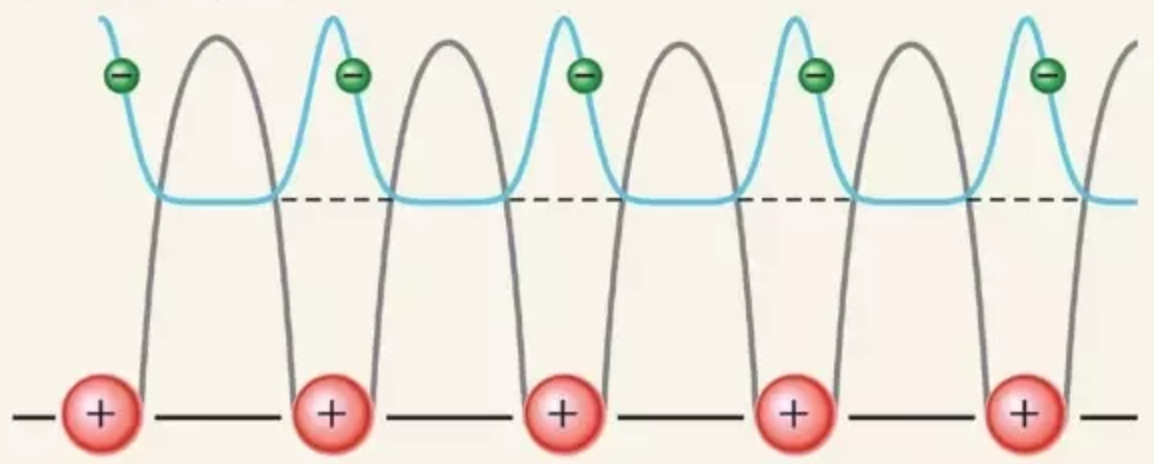
\includegraphics[scale=0.5]{TightBoundModel1.png}
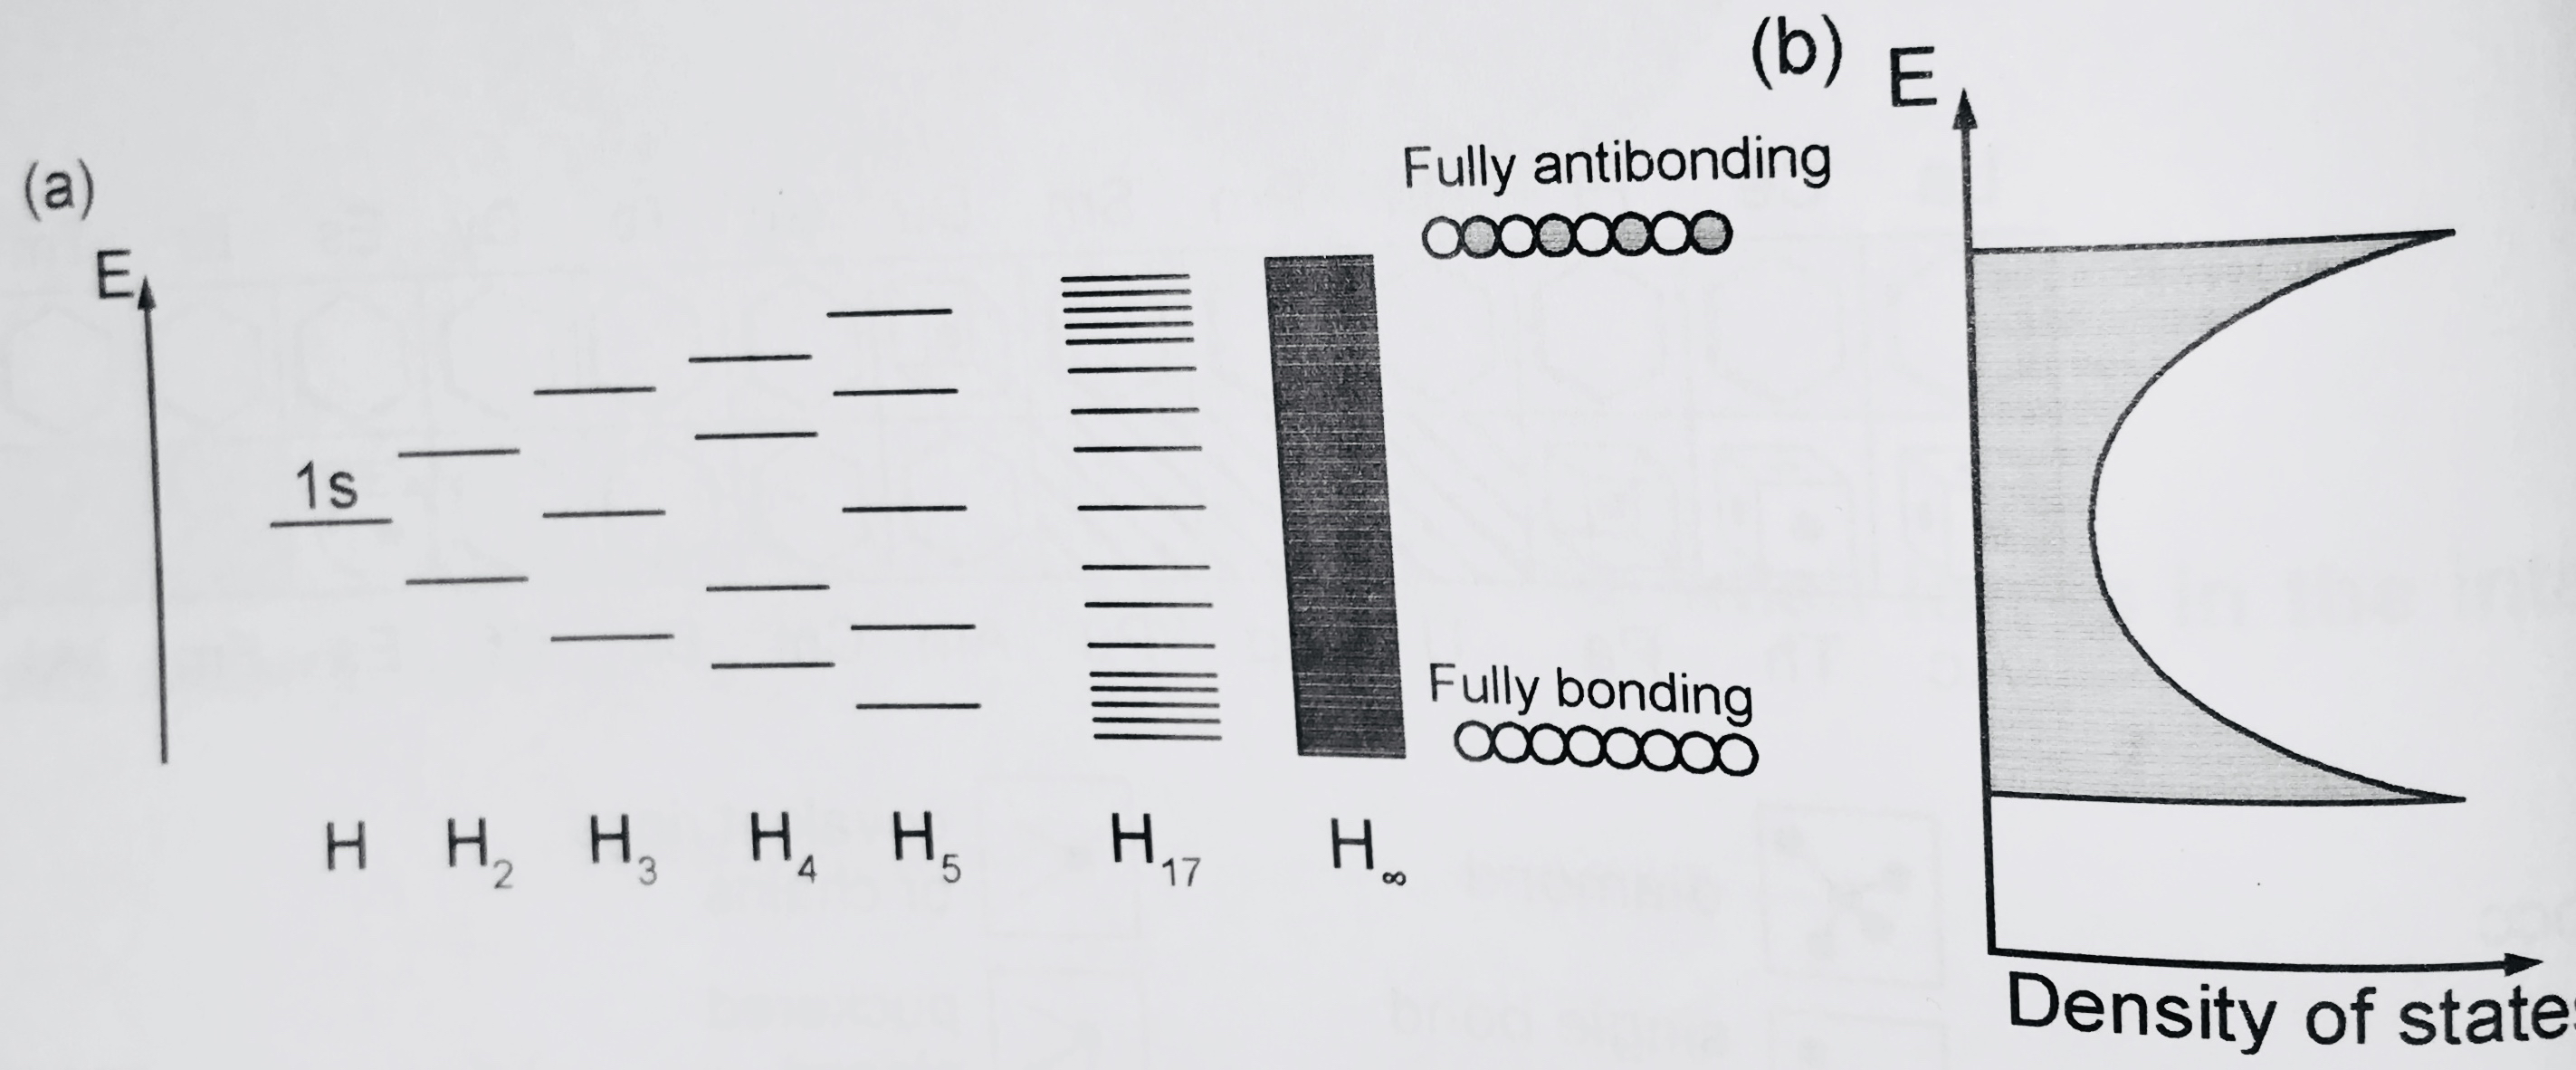
\includegraphics[scale=0.13]{TightBoundModel2.png}
\caption[Tight Bound Model]{Tight Bound Model aplicat a l'estructura electrònica d'un metall. A dalt: podem considerar que cada electró està fortament lligat al seu nucli. A baix: estructura electrònica de considerar un conjunt molt gran d'àtoms d'hidrogen formant un hipotètic cristall metàl·lic; la suma dels orbitals electrònics forma un orbital molecular  amb un continu d'energies \citep{yen_chemistry_2008}.}
\label{fig:TightBoundModel}
\end{figure}

Els electrons disposats d'aquesta manera ocupen orbitals atòmics que es combinen linealment seguint la teoria LCAO (la veurem més endavant) i generen el mateix nombre d'orbitals moleculars. En el cas d'un hipotètic cristall d'àtoms d'hidrogen obtindríem un diagrama energètic dels diferents orbitals fins a formar una banda com es mostra en la part inferior de la Figura \ref{fig:TightBoundModel}.

Un millor model és l'anomenat de l'electró lliure. 
En aquest model, es considera que els electrons es poden moure lliurement per l'estructura tridimensional del metall. 
Així, la quantitat d'electrons $N$ de massa $\mu$ que poden ser encabits en un nivell d'energia $E_{max}$ en un cub tridimensional de costat $a$ ve donat per:
\[
N=\frac{8 \pi a^3}{3} \left( \frac{2 \mu E_{max}}{h^2} \right)^{\frac{3}{2}}
\]
o, dit d'una altra manera, l'energia d'una determinada densitat d'electrons $\rho$ és:
\[E_{max} = \frac{h^2}{2 \mu} \left( \frac{3 \rho}{8 \pi} \right)^{\frac{2}{3}}\]

\begin{figure}[h]
\centering
\includegraphics[scale=0.08]{FreeElectron.png}
\caption[Model de l'electró lliure]{En el model de l'electró lliure, la densitat d'estats d'un gas d'electrons és proporcional a l'arrel quadrada de l'energia cinètica de les partícules \citep{yen_chemistry_2008}. }
\label{fig:FreeElectron}
\end{figure}

A 0K els electrons només ocupen els estats d'energia més baixos fins a l'anomenat nivell de Fermi (Figura \ref{fig:FreeElectron}). Els electrons addicionals que entrin al sistema a causa de la conducció elèctrica omplen els orbitals vacants.

Entre els orbitals ocupats i els orbitals vacants pot existir un gap que fa que a baixa temperatura aquests metalls no condueixin. Es necessita major temperatura per tal que tornin a ser conductors. 
És el que s'anomena un semiconductor. Veure Exercici \ref{Ex:Fermi}.

\begin{exr}
La funció de Fermi $f(E)$ dóna la probabilitat de que un determinat estat energètic sigui ocupat a una determinada temperatura superior a 0K:
\[f(E)=\left( 1 + \exp \left[ \frac{E-E_f}{k_B T} \right] \right)^{-1}\]
a) Dibuixa $f(E)$. b) Si el nivell de Fermi per al coure és de 7eV, raona com es distribuiran els seus electrons a 0K i a 1000K.
\label{Ex:Fermi}.
\end{exr}

\begin{figure}[h]
\centering
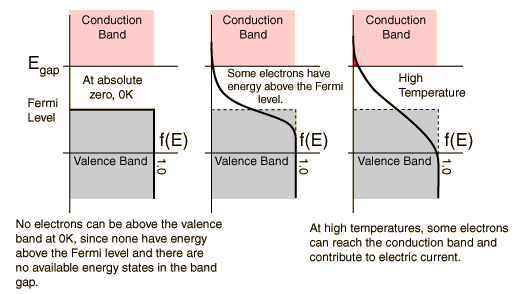
\includegraphics[scale=0.7]{FermiBand.png}
\caption{Efecte de la temperatura en un semiconductor.}
\label{fig:FermiBand}
\end{figure}

\paragraph{Cristalls iònics}
 Cada ió està lligat per una força Coulòmbica als altres i això fa que tinguin energies de dissociació (lattice energies) molt altes. 
\begin{equation}
U=-k\frac{Q_1 Q_2}{r_0} = \frac{NMz_+z_-e^2}{4\pi \varepsilon_0 r_0}
\label{Eq:Coulomb}
\end{equation}
Les energies depenen de la càrrega.
A l'Equació \ref{Eq:Coulomb}, M és l'anmenada constant de Madelung, que és fruït de considerar la interacció amb tota la resta d'ions que ocupen determinades posicions en la retícula.
\begin{figure}[h]
\centering
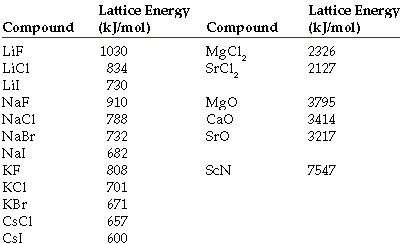
\includegraphics[scale=0.8]{latticeEnergy.png}
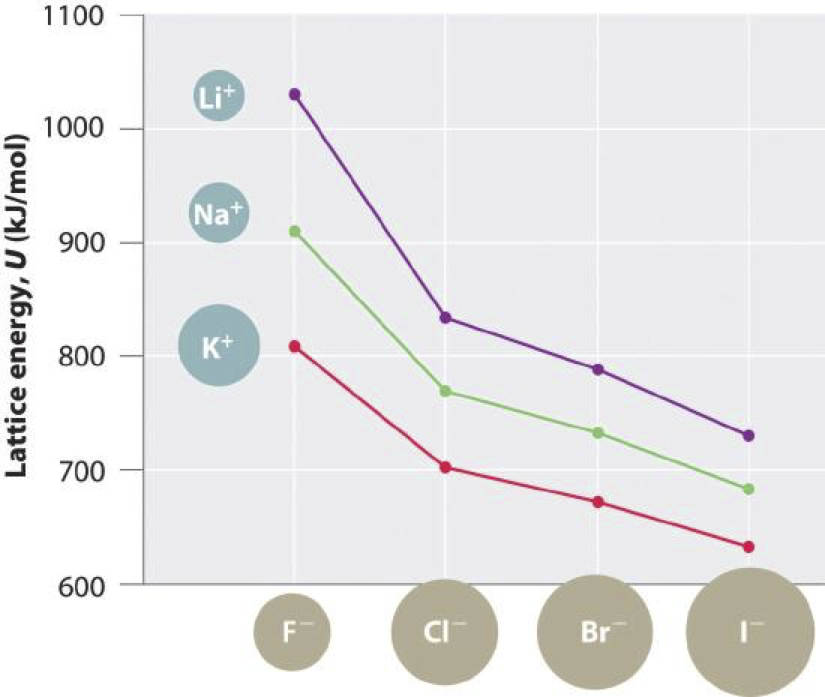
\includegraphics[scale=0.6]{latticeEnergySize.png}
\caption{Energies reticulars (lattice energies) de diversos sòlids iònics.}
\label{fig:latticeEnergy}
\end{figure}
\begin{exr}
Ordena GaP, BaS, CaO, and RbCl per ordre de les seves energies de dissociació.
\end{exr}

\begin{exr}
Usant la descripció del Cicle de Born-Haber que trobaràs a la Wikipedia (\linkurl{https://ca.wikipedia.org/wiki/Cicle_de_Born-Haber}) calcula l'energia reticular del Fluorur de Liti.
\end{exr}

\paragraph{Cristalls moleculars}

Formats per molècules covalents. 
\begin{itemize}
\item[no polars] Es mantenen units per forces de van der Waals de tipus dispersius.
\item[polars] Es mantenen units per unions de vdW dipol-dipol.
\item[ponts d'hidrogen] 
\end{itemize}  

\paragraph{Sòlids covalents}

Tots els àtoms estan units per enllaços covalents (diamant, grafit). Veurem en seccions properes com es formen aquests enllaços.


\begin{exr}
Compara, per als diferents tipus de sòlids descrits, les següents característiques:
\begin{enumerate}
\item pressió de vapor
\item punt de fusió
\item punt d'ebullició
\item duresa
\item fragilitat
\item conducció elèctrica en estat sòlid
\item conducció elèctrica en estat líquid
\end{enumerate}
\end{exr}

\subsection{Defectes}

Les xarxes cristal·lines  incorporen gran nombre de defectes que, sovint, els donen les seves propietats més interessants. Hi ha diversos tipus de defectes en els cristalls:
\begin{description}
\item[Defectes de punt] Impliquen una sola posició (veure Figura \ref{fig:DefectesPunt}). Identifiquem els defectes de Schottky com aquells on apareixen vacants catió-anió en parelles. En un defecte de Frenkel, en canvi, hi ha un desplaçament d'un catiuó cap a una posició intersticial. En els dos casos es manté la neutralitat de l'estructura (a la fluorita, per exemple, els intersticis són grans, i per tant és fpacil trobar defectes de Frenkel). Si el defecte és l'absència d'un anió podem tenir un defecte de tipus centre F.
\item[Defectes de línea] Tenen a veure amb desplaçaments o alteracions d'una fila de posicions a la xarxa. Es poden provocar dislocacions d'aresta (de l'ordre de 10$^6$ per cm$^2$ en un metall templat o 10$^{12}$ per cm$^2$ en un metall treballat en fred.
\item[Defectes de pla] Bidimensionals. Els àtoms en l'extrem dels microcristalls poden ser més reactius per estar exposats amb més facilitat.
\end{description}

\begin{figure}[h]
\centering
\includegraphics[scale=0.1]{DefectesPunt.png}
\caption{Diversos tipus de defecte de punt en un cristall.}
\label{fig:DefectesPunt}
\end{figure}

\begin{exr}
El coure té una estructura cúbica de cara centrada, i l'aresta de la cel·la unitària és de 3.61${\AA}$. Pots suggerir algun tipus d'àtom que es pugui col·locar en els  intersticis de la seva xarxa sense distorsionar-la?
\end{exr}

\begin{exr}
Si la densitat del clorur sòdic sense defectes és de 2.165 g cm$^{-3}$, quina seria la densitat si tingués un ratio de 10$^{-3}$ defectes de a) Frenkel; b) Schottky. (el volum no varia amb els defectes)
\end{exr}

%\subsection{Propietats tèrmiques (M)}

\section{Líquids i dissolucions}

\subsection{Teoria cinètica (M)}

Les partícules que conformen un líquid es poden moure en el seu sí, i Robert Brown (1827) va suggerir que feien de forma aleatòria. Això era degut a la petita mida de les partícules (de l'ordre de 10${-6}$m) i el constant xoc de les partícules que el formen.

\begin{figure}[h]
\centering
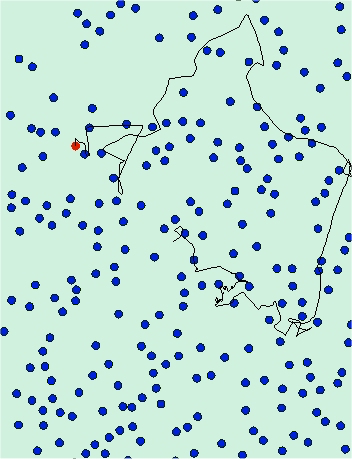
\includegraphics[scale=0.5]{Brownian_motion.png}
\caption[Moviment Brownià]{Representació del moviment Brownià d'una partícula petita en un fluïd. La seva mida fa que els xocs amb les molècules del fluïd faci variar la seva trajectòria de forma globalment aleatòria.}
\label{fig:Brownian_motion}
\end{figure}

El moviment Brownià es pot representar per un model estocàstic en el qual els canvis de posició des d'un instant a l'altre estan produïts per moviments aleatoris extrets d'una distribució normal amb mitjana $\mu=0.0$ i variança $\sigma^2 \times \Delta t$, o $N(0,\sigma^2 \times \Delta t)$. En altres paraules, la variança augmenta amb el temps de forma lineal amb pendent $\sigma^2$. 

\begin{exr}
Usant R, prova d'executar aquest script que mostra com simular el moviment Brownià d'una partícula en un líquid (extret de \linkurl{http://www.phytools.org/eqg/phytools/}):
\begin{lstlisting}[language=R]
t <- 0:100  # temps de simulacio
sig2 <- 0.01
## primer, calcula un conjunt de desviacions aleatòries puntuals
x <- rnorm(n = length(t) - 1, sd = sqrt(sig2))
## després, acumula'n els resultats
x <- c(0, cumsum(x))
plot(t, x, type = "l", ylim = c(-2, 2))
\end{lstlisting}

Després, executa el següent script, que produeix 10000 simulacions diferents:

\begin{lstlisting}[language=R]
nsim <- 1000
## creo una matriu que hostatgi totes les simulacions
X <- matrix(0, nsim, length(t))
for (i in 1:nsim) X[i, ] <- c(0, cumsum(rnorm(n = length(t) - 1, sd = sqrt(sig2))))
plot(t, X[1, ], xlab = "temps", ylab = "desviacions", ylim = c(-2, 2), type = "l")
for (i in 1:nsim) lines(t, X[i, ])
\end{lstlisting}
\end{exr}
\begin{exr}
Per saber la variança que s'obté de la simulació podem fer
\begin{lstlisting}[language=R]
var(X[, length(t)])
\end{lstlisting}
i per mostrar l'histograma de posicions finals:
\begin{lstlisting}[language=R]
hist(X[, length(t)])
\end{lstlisting}
o bé:
\begin{lstlisting}[language=R]
plot(density(X[, length(t)]))
\end{lstlisting}
Calcula la variança de la distribució per a diferents valors del nombre de simulacions o el temps simulat.
\end{exr}

A partir de la teoria cinètico-molecular es pot veure que l'energia mitjana de les partícules en un moviment Brownià és $3/2 RT$, la mateixa que la de les molècules d'un gas a la mateixa temperatura. Només cal pensar en què passa en la interfície d'un líquid i un gas a la mateixa temperatura.


\subsection{Equilibris de fase (M)}

El pas de líquid a vapor s'anomena \emph{vaporització}, i es pot donar a la superfície del líquid (\emph{evaporització}) o en tot el seu volum (\emph{ebullició}).
Es tracta d'un procés endotèrmic. El seu procés contrari és la \emph{condensació}.

\begin{exr}
Explica, segons la teoria cinètico-molecular, la Figura \ref{fig:evap_vs_condens}. Com interpretes els termes \emph{equilibri dinàmic} i \emph{saturació}?
\end{exr}
\begin{figure}[h]
\centering
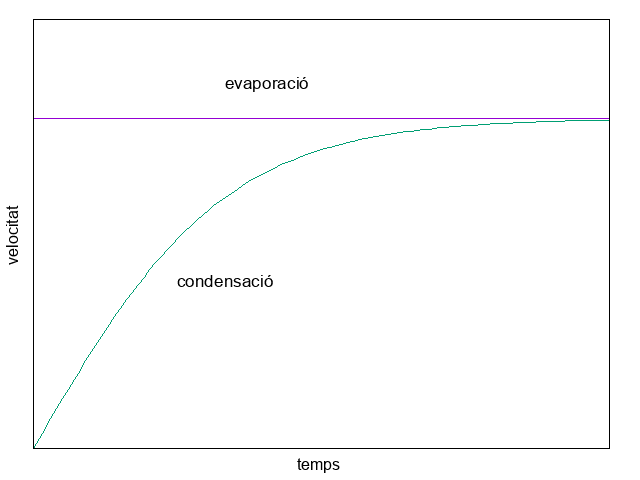
\includegraphics[scale=0.6]{evap_vs_condens.png}
\caption{Esquema de la dependència de les velocitats d'evaporació i condensació respecte el temps en un líquid que s'evapora dins d'un recipient tancat.}
\label{fig:evap_vs_condens}
\end{figure}

La pressió que exerceix el vapor d'una substància a una temperatura determinada un cop és en equilibri amb la mateixa substància líquida és el que anomenem \emph{pressio de vapor} d'aquesta substància, $p_v$. La pressió de vapor augmenta en augmentar $T$, com es veu a la Figura \ref{fig:Water_vapor_pressure_graph}. Tots els líquids presenten corbes similars, amb pendent positiva.

\begin{figure}[h]
\centering
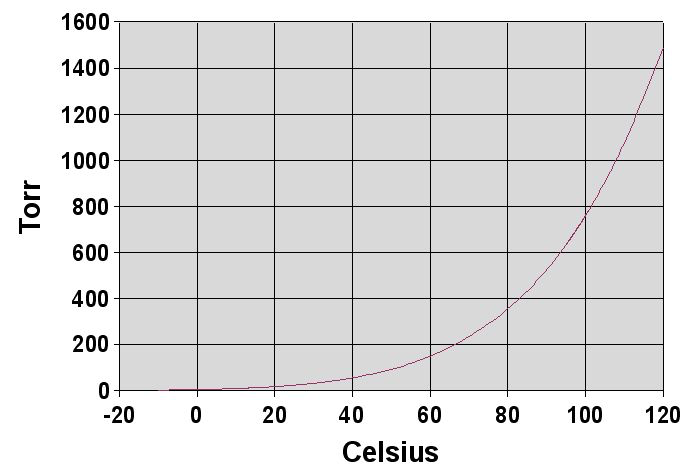
\includegraphics[scale=0.4]{Water_vapor_pressure_graph.png}
\caption{Pressió de vapor de l'aigua en funció de la temperatura.}
\label{fig:Water_vapor_pressure_graph}
\end{figure}

La \emph{temperatura d'ebullició normal} és la que presenta un líquid a pressió 1 atm. La temperatura d'ebullició d'un líquid dependrà de la pressió exterior i de la natura del líquid.

\begin{exr}
És possible que un líquid arribi a estar sobreescalfat: temperatura superior a la d'ecullició per a aquella pressió però encara estat líquid, la qual cosa succeeix quan és molt pur i no hi ha partícules de pols.
Com aconseguiries que no es produeixi aquest sobreecalfament?
\end{exr} 

Hi ha una relació força directa entre la  pressió de vapor, la temperatura d'ebullició i la calor de vaporització (veure Taula \ref{tab:pv}). En general, com més intenses són les force sintermoleculars més alta és $\Delta H_v$ i $T_e$.
\begin{table}[h!]
  \begin{center}
    \caption{Pressió de vapor a 20$\degree$C, temperatura d'ebullició i calor de vaporització d'alguns líquids  (adaptat de \citep{caamano_ros_quimica_1991}).}
    \label{tab:pv}
    \begin{tabular}{ccccc}
%    \begin{tabular}{ccS[table-format=2.4]S[table-format=4.1S[table-format=2.4]}
      \hline
      Líquid & naturalesa & $p_v$/10$^5$Pa & $T_e$/$\degree$C & $\Delta H_v$/kJ mol$^{-1}$\\
      \hline
      \ch{He} & no polar & $-$ & -268.9 & 0.1003 \\
      \ch{H2} & no polar & $-$ & -252.7 & 0.9028 \\
      \ch{CH4} & no polar & $-$ & -161.4 & 9.263 \\
      \ch{n-C4H10} & no polar & 2.03 & -1.5 & 24.24 \\
      \ch{CCl4} & no polar & 0.121 & 76.7 & 34.57 \\
      \ch{NH3} & polar & 10.1 & -33-6 & 20.15 \\
      \ch{H2O} & polar & 0.0233 & 100.0 & 40.62 \\
      \ch{CH3CH2OH} & polar & 0.0586 & 78.5 & 40.44 \\
      \ch{CH3OCH3} & polar & 5.06 & -23.7 & 22.61 \\
      \ch{CH3COCH3} & polar & 0.247 & 56.5 & 31.94 \\
      \hline
    \end{tabular}
  \end{center}
\end{table}

La Figura \ref{fig:hidrurs_boiling_point} mostra com la $T_e$ evoluciona en paral·lel a la taula periodica, i també com algunes substàncies són significativament excepcions d'aquesta norma degut a la seva capacitat d'establir ponts d'hidrogen.
\begin{figure}[h]
\centering
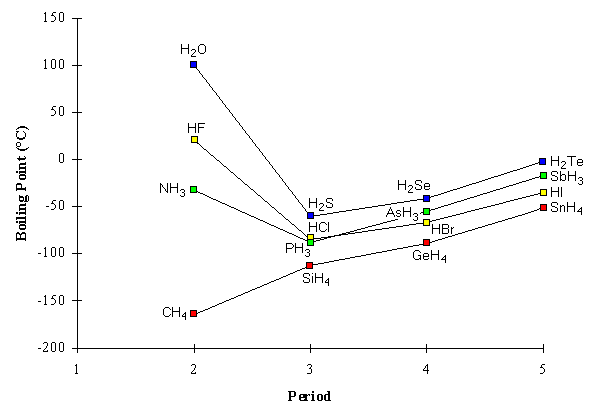
\includegraphics[scale=0.4]{hidrurs_boiling_point.png}
\caption{Punts d'ebullició de diversos hidrurs relacionats amb la posició dels seus elements no metàl·lics a la taula periòdica.}
\label{fig:hidrurs_boiling_point}
\end{figure}

\subsection{Propietats crítiques}
\label{sec:PropietatsCritiques}

Michael Faraday va licuar gas clor el 1823, però per a altres gasos (\ch{H2}, \ch{N2} o \ch{O2}) no es va aconseguir i no va ser fins que Thomas Andrews va aconseguir liquar \ch{CO2} només si treballava a temperatures inferiors a 31$\degree$C. Així va sorgir el concepte de \emph{temperatura crítica}, $T_c$, com a propietat característica dels gasos, i que es defineix com aquella a partir de la qual no és possible liquar-los (veure Figura \ref{fig:punt_critic}).
En el punt crític, la $P_c$ és la pressió de vapor del líquid a $T_c$. És la màxima pressió de vapor del líquid, ja que a més $T$ no té sentit parlar-ne, ja que no existeix l'estat líquid. La corba de pressió front a la temperatura finalitza, doncs, en aquest punt.

\begin{figure}[h]
\centering
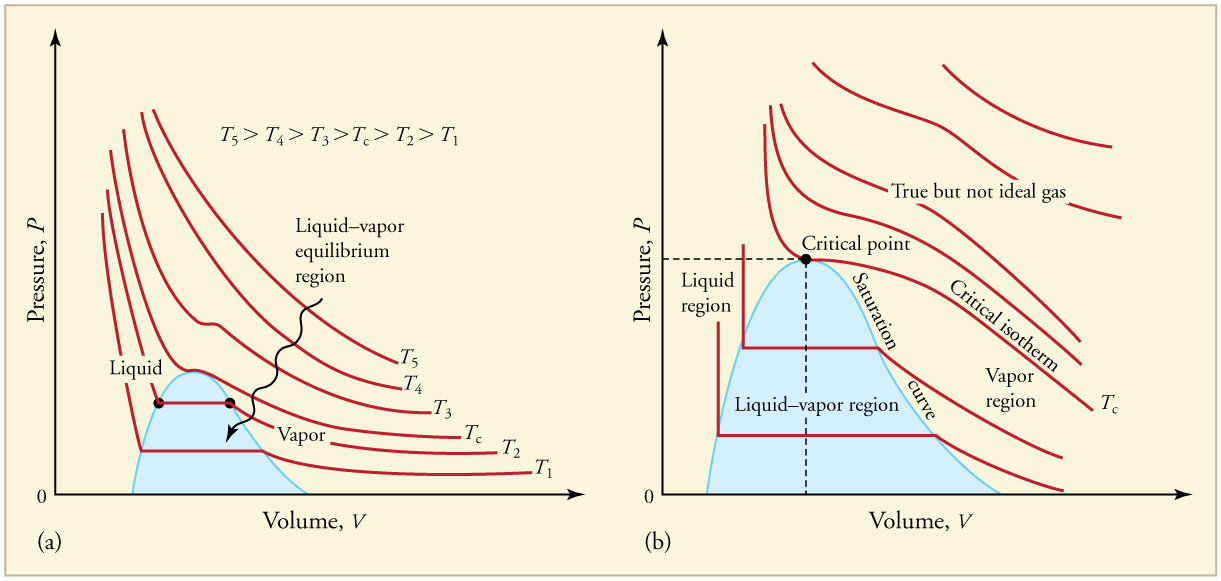
\includegraphics[scale=0.6]{punt_critic.png}
\caption[Punt crític]{a) Cada corba isoterma representa la relació entre $P$ i $V$ a una temperatura donada. Les corbes inferiors deixen de sser hipèrboles perquè el gas es torna no ideal; b) el terme ``vapor'' es refereix a gas a una temperatura inferior al punt d'ebullició. Veure valors de punts crítics de substpancies comunes a \linkurl{http://philschatz.com/physics-book/contents/m42218.html}.\citep{openstax_cnx_openstax_nodate}}
\label{fig:punt_critic}
\end{figure}


\begin{figure}[h]
\centering
\includegraphics[scale=0.8]{WaterPD.png}
\caption[Diagrama de fases simplificat de l'aigua]{Diagrama de fases simplificat de l'aigua. El gràfic no és a escala i tampoc conté diverses variants específiques que el farien molt complex.\citep{openstax_cnx_openstax_nodate}}
\label{fig:WaterPD}
\end{figure}
Al PC, la concentració molecular i tota la resta de propietats es fan iguals per al líquid i el gas.

\begin{exr}
Què ens produirà una cremada més gran: una massa $m$ d'\ch{H2O}(g) a 100 graus o la mateixa quantitat d'aigua líquida a la mateixa temperatura?
\end{exr}

\begin{exr}
En un recipient hi ha aigua líquida. Es conecta el frecipient a una bomba de buit i es va abaixant la pressió sobre el líquid. Si la temperatura és de 60 graus, a quina pressió bullirà l'aigua?
\end{exr}

\begin{exr}
Perquè a la Taula \ref{tab:pv} no apareix la $p_v$ de l'\ch{He}, \ch{H_2} i \ch{CH4}?
\end{exr}

A partir de tot el què hem treballat fins a aquest punt, queda clar que hi ha dues forces motores dels processos moleculars. D'una banda tots tendeixen a la mínima energia, però això no explicaria perquè els gasos existeixen com a tals. És necessari considerar la necessitat de tendir a un màxim desordre. El primer efecte ve determinat per l'entalpia del sistema i el segon per l'entropia. Ho treballarem més endavant amb major detall.

Ara com ara sí que podem, però determinar quatre característiques importants que tornarem a retrobar i formular:
\begin{enumerate}
\item L'equilibri en els sistemes moleculars és dinàmic, conseqüència de velocitats de reacció oposades.
\item El sistema passa espontàniament a l'estat d'equilibri.
\item Un cop assolit l'equilibri, les seves propietats són sempre les mateixes.
\item L'equilibri és fruit de dues tendències oposades: la necessitat d'assolir el mínim d'energia i la tendència al màxim caos.
\end{enumerate}

Això es pot escriure en base a l'energia lliure del procés d'equilibri. En equilibri, $\Delta G=\Delta H - T\Delta S0$, i per a tot procés espontani, $\Delta G <0$.
Més endavant anirem ampliant aquests conceptes termodinàmics, però ara com ara ens serveixen per entendre els fenòmens que hem anat explornat i que veure a continuació.

\subsection{Dissolucions}

Una dissolució és una substància complexa homogènia que, dins d'uns límits raonables, té una composició que pot variar contínuament.
Veurem més endavant que aquesta definició no és massa clara (pensem en el sabó en l'aigua).

La mesura de la concentració d'una dissolució pot donar-se en:
\begin{itemize}
\item \emph{Unitats de fracció molar.} $x_1=\frac{n_1}{n_1+n_2}$ i $x_2=\frac{n_2}{n_1+n_2}$
\item \emph{Molalitat} Número de mols de solut que hi ha en 1000g de solvent.
\item \emph{Molaritat} Número de mols per 1 litre de dissolució.
\item \emph{Normalitat} Número de pesos equivalents-gram del solut en un litre de dissolució.
\end{itemize}
\subsection{Solucions ideals i no ideals}

\begin{exr}
Raona com canvia la $p_v$ d´'una dissolució en funció de la seva concentració.
\end{exr}
Una dissolució ideal es forma sense despreniments de calor i amb una pressio de vapor que evoluciona segons la llei de Raoult:
\[
P_{dissolució}=P_{dissolvent}=P_1=P_1^0x_1 = P_1^0 \left(\frac{n_1}{n_1+n_2}\right)
\]
\begin{exr}
Determina la relació entre l'increment de pressió de vapor d'una dissolució i la fracció molar del solut.
\end{exr}
\begin{exr}
La pressió de vapor de l'aigua a 20$\degree$C és 17.54 mmHg. Quan dissolem 114g de sucrosa en 1000g d'aigua, la pressió de vapor es redueix en 0.11 mmHg. Quin és el pes molecular de la sucrosa?
\end{exr}

A partir de la llei de Raoult es pot arribar amb relativa facilitat a una expressió que relaciona la molalitat amb l'increment del punt d'ebullició:
\[
\Delta T=K_b m
\]
on $K_b$ és la constant d'elevació molal del punt d'ebullició respecte la concentració.
\begin{exr}
a) Exactament 1.00g d'urea dissolts en 75.00g d'aigua donen una dissolució que bull a 100.114$\degree$C. El pes molecular de la urea és 60.1. Quina és la $K_b$ de l'aigua?
b) Una dissolució preparada dissolent 12,00g de glucosa en 100g d'aigua bull a 100.34$\degree$C. Quin és el pes molecular de la glucosa?
\end{exr}
Quelcom similar es pot deduir per al punt de fusió: \[\Delta T = K_f m\]. Cal notar que, si en lloc de només un solut n'hi ha més d'un, hem de tenir en compte la molalitat total de la dissolució.

En el cas de tenir més d'un component volàtil a la dissolució, només hem de tenir present que la llei de Raoult s'acomplirà per a totes dues, i per tant la pressió parcial de cadascuna de les dues substàncies volàtils s'haurà de sumar:
\[
P_T=P_1+P_2=x_1P_1^0+x_2P_2^0
\]

En una dissolució ideal de dues components, el vapor sempre es troba enriquit amb aquella de les dues substàncies que sigui més volàtil.
A partir de la diferència de volatilitat de dos components en una dissolució podem analitzar la composició del vapor fent servir diagrames com el de la Figura \ref{fig:PhaseDiagram}a.
Usant aquesta mena de diagrames podem estudiar la destil·lació fraccionada d'una dissolució líquida de dues substàncies volàtils (Figura \ref{fig:PhaseDiagram}b).

\begin{figure}[h]
\centering
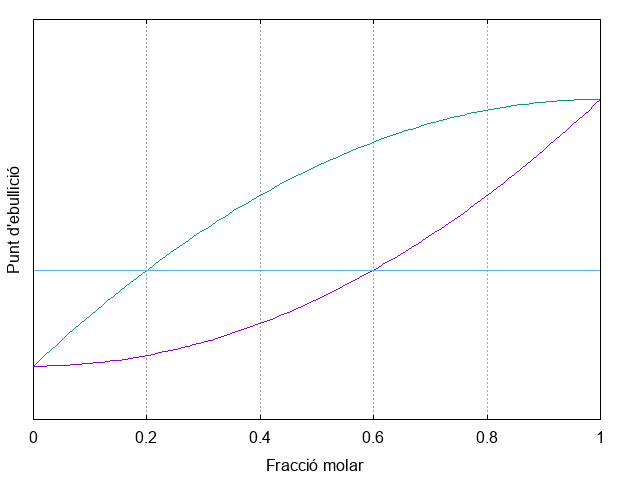
\includegraphics[scale=0.5]{PhaseDiagram.png}
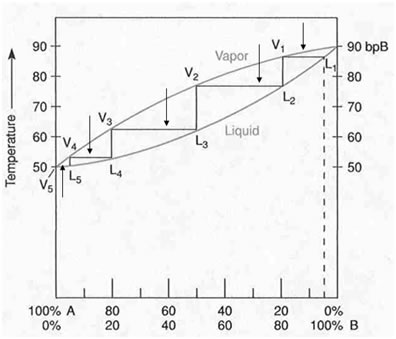
\includegraphics[scale=0.5]{FractionalDistillation.png}
\caption[Diagrama de fases i destil·lació fraccionada d'una dissolució ideal]{a) La corba inferior mostra el punt d'ebullició d'una dissolució ideal per a diferents composicions. La corba superior mostra la composició del vapor, si connectem, per a una $T_{ebullició}$ d'ebullició donada, els punts de tall de les dues corbes a aquesta $T$. b) Destil·lació fraccionada d'una disslució ideal.}
\label{fig:PhaseDiagram}
\end{figure}

En una dissolució ideal no es desprèn ni absorbeix calor ($\Delta H=0$) i per tant, el procés és purament entròpic, cosa que el fa espontani (si $\Delta H=0$, $\Delta G= -T \Delta S<0$).

En dissolucions no ideals, observem una desviació respecte la llei de Raoult que pot ser positiva o negativa (veure, per exemple, \linkurl{https://www.youtube.com/watch?v=4hmrDSxEN-Q} o la Figura \ref{fig:desv_raoult}).
\begin{figure}[h]
\centering
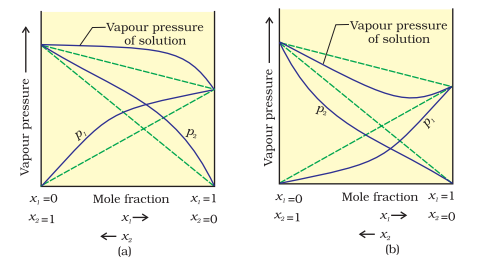
\includegraphics[scale=1.0]{desv_raoult.png}
\caption[Llei de Raoult per dissolucions ideals i no ideals]{a) en una desviació positiva respecte la llei de Raoult, els dos líquids que formen la barreja les forces d'atracció entre les dues substàncies són menors que les que es produeixin dins d'una d'elles: A i B escapen fàcilment i mostren, per tant, major pressió de vapor que l'esperada; b) en una desviació negativa, els dos líquids mostren una atracció mútua més gran que en cadascun per separat: les substàncies A i B tendeixen a marxar de la dissolució menys que en la situació ideal.}
\label{fig:desv_raoult}
\end{figure}

És interessant separar les dissolucions entre aquelles que:
\begin{itemize}
\item Desprenen calor en formar-se ($\Delta H <0$). Per exemple, si dissolem cloroform (\ch{CHCl3}) en acetona (\ch{(CH3)2CO}), es desprèn calor, en tant que es formen ponts d'hidrogen entre les molècules dels dos tipus de substància, però no dins de cadascuna d'elles (veure Figura \ref{fig:CloroformAcetona}).
\begin{figure}
  \centering
\chemfig{Cl>:[,1.2]C(<[3,1.2]Cl)(<[5,1.2]Cl)(-[0]H-[,,,,dash pattern=on 2pt off 2pt]O=C(-[1]CH_3)(-[7]CH_3))}
(\cmpd{cpmd:CloroformAcetona})\par
  \caption{La interacció de pont d'hidrogen entre el cloroform i l'acetona provoca un comportament no ideal de la llei de Raoult.}
  \label{fig:CloroformAcetona}
\end{figure}
En aquest cas, la pressió de vapor serà menor a l'esperada a partir de la llei de Raoult (Figura \ref{fig:desv_raoult}b). 
\item Absorbeixen calor en formar-se ($\Delta H > 0$). Això succeeix en els casos en els què barregem sbstàncies polars amb no polars i, per tant, eliminem moltes interaccions que altrament ja serien prou favorables. Per exemple, si barregem acetona (veure estructura a \ref{cpmd:ClorofomAcetona}) amb bisulfur de carboni (\chemfig{S=C=S}). Veure Figura \ref{fig:desv_raoult}a)
\end{itemize} 
Per tant, si la $T$ canvia en fer una dissolució de dues substàncies, la dissolució és no ideal.
Si observem amb atenció la Figura \ref{fig:desv_raoult} veiem que en el límit de dilució (dilució infinita) el corresponent dissolvent es comporta de forma propera a la ideal.

En una dissolució no ideal de dos components, a diferència del què passava amb les dissolucions idelas, no sempre el vapor es troba enriquit amb la substància més volàtil. 

\begin{exr}
Raona l'efecte que té la no idealitat de les dissolucions segons la Figura \ref{fig:desv_raoult}a a) en el seu punt d'ebullició, i b) en un procés de destil·lació fraccionada.
\end{exr}

Les dissolucions que destil·len sense canvi en la composició s'anomenen azeòtropes. Per exemple, si fem una barreja d'agua i àcid clorhídric i la fem bullir un temps suficient, la seva composició arribarà a un pes d'\ch{HCl} del 20.22\% respecte el pes total.

\begin{exr}
Un azeòtrop positiu prové d'una desviació també positiva de la llei de Raoult. a) Dibuixa la corba de Temperatura d'ebullició vs composició per a un azeòtrop positiu basant-te en les Figures \ref{fig:PhaseDiagram}a i \ref{fig:desv_raoult}a. b) Raona el resultat de fer una destil·lació a partir de diverses composicions d'aquesta mescla. c) què succeiria en un azeòtrop negatiu?
\end{exr}
\begin{figure}[h]
\centering
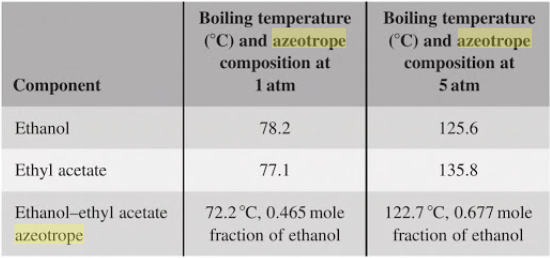
\includegraphics[scale=1.0]{AzeotropEX.png}
\caption{Dades per al sistema etanol - acetat etílic (extret de \citep{Robin2016}).}
\label{fig:AzeotropEX}
\end{figure}
\begin{exr}
Volem separar una barreja equimolar d'etanol i acetat etílic per destil·lació en productes relativament purs. La barreja forma un azeòtrop de mínim punt d'ebullició segons la Figura \ref{fig:AzeotropEX}. No obstant, la composició de l'azeòtrop és sensible a la pressió, mostrant un increment significatiu de la fracció molar de l'etanol quan incrementa la pressió, com es mostra a la Figura. Dibuixa un esquema aproximat per a la separació de les dues components de la barreja que tregui profit d'aquest fet.
\end{exr}

\subsection{Solubilitat}

En la majoria dels casos, dues substàncies no es poden dissoldre l'una en l'altra en qualsevol proporció.
La solubilitat d'una substància en un determinat dissolvent, a una temperatura donada, és la concentració del solut en la dissolució saturada.
És una propietat fonamental per separar components d'una dissolució.
La solubilitat depèn de la natura de dissolvent i solut, així com de la $T$ i la $P$.

Per entendre l'efecte de la $T$ en la solubilitat usarem l'anomenat principi de LeChatelier, segons el qual "si s'exerceix alguna acció sobre un sistema que inicialment està en equilibri que afecti algun dels factors que l'identifiquen com a tal, el sistema es regularà ell mateix de manera que tendeixi a reduir l'efecte d'aquell canvi".
\begin{exr}
Raona perquè per a una dissolució en la qual $\Delta H_{sol} <0$, un augment de la temperatura fa que la solubilitat disminueixi, i a l'inrevés.
\end{exr}

%test

Es pot relacionar les pressió d'un gas i la seva solubilitat a una $T$ donada en un líquid segons la llei de Henry\marginnote{William Henry, 1775-1836}:
\[
C=kP
\]
on $C$ és la concentració (M) del gas en el líquid, $P$ la pressió parcial del gas i $k$ la constant de Henry, que depèn de la $T$ i la natura de gas i dissolvent (veure Taula \ref{tab:Henry}).

\begin{table}[h!]
  \begin{center}
    \caption{Constants de la llei de Henry per a diferents gasos en aigua a 20$\degree$C.}
    \label{tab:Henry}
    \begin{tabular}{cc}
      \hline
      Gas & constant de Henry / mol l$^{-1}$ atm$^{-1}$ \\
      \hline
He &	3.9\\
Ne &	4.7\\
Ar &	15\\
H2 &	8.1\\
N2 &	7.1\\
O2 &	14\\
CO2& 	392\\      
      \hline
    \end{tabular}
  \end{center}
\end{table}
